%
% File acl2018.tex
%
%% Based on the style files for ACL-2017, with some changes, which were, in turn,
%% Based on the style files for ACL-2015, with some improvements
%%  taken from the NAACL-2016 style
%% Based on the style files for ACL-2014, which were, in turn,
%% based on ACL-2013, ACL-2012, ACL-2011, ACL-2010, ACL-IJCNLP-2009,
%% EACL-2009, IJCNLP-2008...
%% Based on the style files for EACL 2006 by 
%%e.agirre@ehu.es or Sergi.Balari@uab.es
%% and that of ACL 08 by Joakim Nivre and Noah Smith

\documentclass[11pt,a4paper]{article}
\usepackage{authblk}
\usepackage{blindtext}
% \usepackage[draft]{hyperref}
\usepackage[hyperref]{acl2018}
\usepackage{times}
\usepackage{latexsym}
\usepackage{qtree}
\usepackage{graphicx}
\usepackage{amsmath}
\usepackage{amsfonts,amssymb}
\usepackage{multirow}
\usepackage{multicol}
\usepackage{enumitem}
\usepackage{comment}
\usepackage{url}

\aclfinalcopy % Uncomment this line for the final submission
\def\aclpaperid{760} %  Enter the acl Paper ID here

%\setlength\titlebox{5cm}
% You can expand the titlebox if you need extra space
% to show all the authors. Please do not make the titlebox
% smaller than 5cm (the original size); we will check this
% in the camera-ready version and ask you to change it back.
\newcommand{\matr}[1]{\mathbf{#1}}
\renewcommand{\vec}[1]{\mathbf{#1}}

\newcommand{\figref}[1]{Figure \ref{#1}}
\newcommand{\tabref}[1]{Table \ref{#1}}
\newcommand{\secref}[1]{Section \ref{#1}}
% \newcommand{\YZ}[1]{\textcolor{purple}{Yizhong: #1}}

\usepackage{etoolbox}
\makeatletter
\patchcmd{\maketitle}
 {\def\@makefnmark}
 {\def\@makefnmark{}\def\useless@macro}
 {}{}
\makeatother
 

\title{Multi-Passage Machine Reading Comprehension \\ with Cross-Passage Answer Verification}


\author[1 *]{Yizhong Wang\thanks{\llap{\textsuperscript{*}}This work was done while the first author was doing internship at Baidu Inc.}}
\author[2]{Kai Liu}
\author[2]{Jing Liu}
\author[2]{Wei He}
\author[2]{\\Yajuan Lyu}
\author[2]{Hua Wu}
\author[1]{Sujian Li}
\author[2]{Haifeng Wang}
\affil[1]{Key Laboratory of Computational Linguistics, Peking University, MOE, China}
\affil[2]{Baidu Inc., Beijing, China}
% \affil[ ]{\texttt{\{yizhong, lisujian\}@pku.edu.cn}}
\affil[ ]{\tt {\{yizhong, lisujian\}@pku.edu.cn, \{liukai20, liujing46, }}
\affil[ ]{\tt {hewei06, lvyajuan, wu\_hua, wanghaifeng\}@baidu.com}}
\renewcommand\Authands{ and }
\date{}

\begin{document}
\maketitle

\begin{abstract}

Machine reading comprehension (MRC) on real web data usually requires the machine to answer a question by analyzing multiple passages retrieved by search engine. 
Compared with MRC on a single passage, multi-passage MRC is more challenging, since we are likely to get multiple confusing answer candidates from different passages.
To address this problem, we propose an end-to-end neural model that enables those answer candidates from different passages to verify each other based on their content representations.
% To address this problem, we propose an end-to-end neural model by leveraging the content representations of the candidate answers to verify each other. 
% Specifically, our model employs joint training and predicting the final answer by combining the confidence scores from three aspects: the answer boundary, the answer content and the cross-passage answer verification. 
Specifically, we jointly train three modules that can predict the final answer based on three factors: the answer boundary, the answer content and the cross-passage answer verification. 
The experimental results show that our method outperforms the baseline by a large margin and achieves the state-of-the-art performance on the English MS-MARCO dataset and the Chinese DuReader dataset, both of which are designed for MRC in real-world settings. 

% Machine reading comprehension (MRC) on real web data usually requires the model to answer the question given multiple passages retrieved by search engines. 
% % Compared with single-passage MRC,  there are probably multiple confusing answer candidates coming from different passages, which are extremely challenging for MRC models to distinguish. 
% Compared with the MRC on single passage, multi-passage MRC is more challenging since there are likely multiple confusing answer candidates coming from different passages.
% In this work, we propose an end-to-end framework that enables those answer candidates from different passages to verify each other based on their content representation. Our model  predicts the final answer from three aspects: the answer boundary, the answer content and the cross-passage answer verification. Experiments show that our method outperforms the baseline model by a large margin and achieves state-of-the-art performance on both the English MS-MARCO dataset and the Chinese DuReader dataset. 
\end{abstract}

\section{Introduction}

Locating visual landmarks, such as human body joints \cite{toshev2014deeppose} and facial key points \cite{xiong2013supervised}, is an important yet challenging problem. The stacked U-Nets, {\it e.g.} hourglasses (HGs) \cite{newell2016stacked}, are widely used in landmark localization. Generally speaking, their success can be attributed to design patterns: 1) within each U-Net, connect the top-down and bottom-up feature blocks to encourage gradient flow; and 2) stack multiple U-Nets in a cascade to refine prediction stage by stage.

However, the shortcut connection exists only ``locally'' inside each U-Net \cite{ronneberger2015u}. There is no ``global'' connection across U-Nets except the cascade. Blocks in different U-Nets cannot share features, which may impede the information flow and lead to redundant parameters.

We propose densely connected U-Nets (DU-Net) to address this issue. The key idea is to directly connect blocks of the same semantic meanings, {\it i.e.} having the same resolution in either top-down or bottom-up context, from any U-Net to all subsequent U-Nets. Please refer to Fig. \ref{fig:framework} for an illustration. The dense connectivity is similar to DenseNet \cite{huang2016densely} but generalizing the design philosophy from feature to semantic level. It encourages information flow as well as feature reuse ``globally'' across the stacked U-Nets, yielding improved localization accuracy. 

Yet there are critical issues in designing DU-Net: 1) The number of parameters would have a quadratic growth since $n$ stacked U-Nets could generate $O(n^2)$ connections. 2) A naive implementation may allocate new memory for every connection, making the training highly expensive and limiting the maximum depth of DU-Nets. 

% The training would be extremely memory expensive since a naive implementation has to make a copy of every connected feature for network forward and back propagation.  



\begin{figure*}[t!]
\centering
  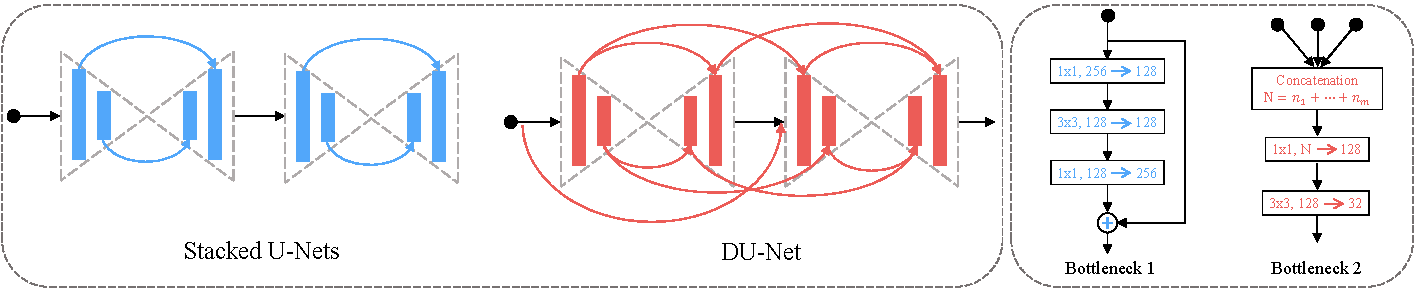
\includegraphics[width=1.0\linewidth]{figures/framework-cropped.pdf}
\caption{Illustration of stacked U-Nets and DU-Net. Stacked U-Nets has skip connections only within each U-Net. In contrast, DU-Net also connects blocks with the same semantic meanings across different U-Nets. The feature reuse could significantly reduce the size of bottleneck in each block, as shown in the right figure. Consequently, with the same number of U-Nets, DU-Net has only 30\% parameters of stacked U-Nets.}
\label{fig:framework}
\end{figure*}

% 
Our solution to those efficiency issues is threefold. {\bf First}, instead of connecting all stacked U-Nets, we only connect a U-Net to its $K$ successors. We name it as the $order$-$K$ connectivity, which aims to balance the fitting accuracy and parameter efficiency by cutting off long-distance connections. {\bf Second}, we employ a memory-efficient implementation in training. The key idea is to reuse a pre-allocated memory so all connected blocks could share the same memory. Compared with the naive implementation, this strategy makes it possible to train a very deep DU-Net (actually, $2\times$ deeper). {\bf Third}, to further improve the efficiency, we investigate an iterative design that may reduce the model size to one half. More specifically, the output of the first pass of the DU-Net is used as the input of the second pass, where detection or regression loss is applied as supervision. 

% %G%
% In view of deploying our approach on mobile devices, we further attempt to quantize weights, inputs, and gradients of DU-Net to low bit-width discrete values. This not only decreases the high precision operations but also shrinks the memory usage during training. By network quantization, the size of trained model can also be largely compressed.
% %G%
Besides shrinking the number of network parameters, we also study to further quantize each parameter. This motivates from the ubiquitous mobile applications. Although current mobile devices could carry models of dozens of MBs, deploying such networks requires high-end GPUs. However, quantized models could be accelerated by some specifically designed low-cost hardwares. Beyond only deploying models on mobile devices \cite{li2017deeprebirth}, training deep neural networks on distributed mobile devices emerges recently \cite{mcmahan2016communication}. To this end, we also try to quantize not only the model parameters but also its inputs (intermediate features) and gradients in training. This is the first attempt to investigate training landmark localizers using quantized inputs and gradients.


In summary, our key contributions are:
\begin{itemize}
    \item To the best of our knowledge, we are the first to propose quantized densely connected U-Nets for visual landmark localization, which largely improves the information flow and feature reuse at the semantic level.
    \item We propose the $order$-$K$ connectivity to balance accuracy and efficiency. It decreases the growth of model size from quadratic to linear by removing trivial connections. Experiments show it could reduce $\sim$70\% parameters of state-of-the-art landmark localizers.
    \item Very deep U-Nets can be trained using a memory-efficient implementation, where pre-allocated memory is reused by all connected blocks.
    \item We further investigate an iterative refinement that may cut down half of the model size, by forwarding DU-Net twice using either detection or regression supervision.
    %G%
    \item Different from previous efforts of quantizing only the model parameters, we are the first to quantize their inputs and gradients for better training efficiency on landmark localization tasks. By choosing appropriate quantization bit-widths for weights, inputs and gradients, quantized DU-Net achieves $\sim$75\% training memory saving with comparable performance. 
    %G%
    \item Exhaustive experiments are performed to validate DU-Net in different aspects. In both human pose estimation and face alignment, DU-Net demonstrates comparable localization accuracy and use $\sim$2\% model size compared with state-of-the-art methods.
\end{itemize}

% We are the first to deploy network quantization for better training efficiency on localization tasks. By choosing appropriate quantization bit-widths for weights, inputs and gradients, quantized DU-Net achieves at least 32$\times$ memory saving with comparable performance to the-state-of-art approaches. 


%The landmark localization such as human pose estimation \cite{toshev2014deeppose,newell2016stacked,wei2016convolutional}, facial landmark localization \cite{xiong2013supervised,zhang2014facial,sagonas2013300}, etc, plays an important role in the higher-level image understanding. The Convolutional Neural Networks (CNNs) have dominated this field, among which recent architecture of stacked hourglasses \cite{newell2016stacked}, a variant of the U-Net \cite{ronneberger2015unet}, becomes a standard solution. The skip connections between top-down and bottom-up blocks within a U-Net could preserve the spatial information and increase the gradient flow. With multiple U-Nets stacked together, the prediction could be refined stage by stage. However, the connections are only within each U-Net of the stacked hourglasses and no explicit connections exist between U-Nets, which may impede the information flow across them. And the blocks with the same semantics in different U-Nets cannot share features, leading to many redundant parameters. 

% Its success attributes to three key factors: repeated top-down, bottom-up inferences, intermediate supervisions and residual bottlenecks \cite{}. 

% The multiple stage top-down and bottom-up processing could better integrate both the local and global visual contexts into the final prediction. The intermediate supervision and residual bottlenecks, on the other hand, could alleviate the gradient vanish problem in deep networks.
%In this paper, we propose to densely connect stacked U-Nets by linking blocks with the same semantics in different U-Nets. We refer to this architecture as {\it Dense U-Nets}. The blocks in a U-Net could get direct inputs from its connected blocks in all preceding U-Nets, making the information flow more efficiently among the U-Nets. The feature reuse at each resolution could reduce the parameters in each block. The dense connectivity in our Dense U-Nets is different from that of DenseNet \cite{huang2016densely}. More specifically, layers only within each single block of the DenseNet are connected. In contrast, we connect blocks lying across the whole Dense U-Nets and connections of hierarchical blocks are mixed together. An illustration is given in Figure \ref{fig:framework}. We name it as the {\it global dense connectivity} to differentiate from the local one in the DenseNet.

% Besides, features in the Dense U-Nets are fused by the concatenation which could facilitate the information flow compared with the summation operation in the stacked hourglasses.

% Although the dense connectivity in our Dense U-Nets is similar with that of DenseNet \cite{}, 
% More recently, the DenseNet \cite{} achieves superior image classification performance over the ResNet \cite{} in terms of both the accuracy and model size, which benefits from the dense connections between layers. Its key insight is the feature reuse between layers of the same resolutions. The dense connectivity in the DenseNet, existing within one block, is local. By extending this principle, we propose a global dense connectivity, in contrast to the local connectivity in \cite{}, that blocks at the same locations of different U-Nets are connected. Hence, we refer to this architecture as {\it Dense U-Nets}. To our best knowledge, we are the first to generalize the local dense connectivity into the stacked U-Nets. 
% The global dense connectivity could make it easier to train much deeper stacked U-Nets.

% This motivates us to replace the residual modules  in the stacked hourglasses with the dense connected layers. However, this dense connectivity exists only locally within a contiguous  block in which all feature maps have the same spatial resolution. A U-Net, on the other hand, consists of a sequence of top-down and bottom-up blocks. A straight way is to turn each block into a dense block with multiple layers. However, this would sacrifice the spirit of stacked hourglasses that multiple stacked hourglasses outperform a single hourglass with multiple layers in each block.

% In order to integrate the structure of stacked U-Nets together with the idea of dense connectivity, we propose a global dense connectivity, in contrast to the local connectivity in \cite{}, that blocks at the same locations of different U-Nets are connected. Hence, we refer to this architecture as {\it Dense U-Nets}. The connected layers in the Dense U-Nets distribute along the whole network rather than in local continuous blocks. Compared with the local residual modules in the stacked hourglasses, the global dense connections could significantly facilitate the gradient to flow across stacked U-Nets.

%In practice, the Dense U-Nets have the efficiency problems of both parameter and training memory. First, suppose a Dense U-Nets contains $n$ U-Nets, there would be $O(n(n-1)/2)$ connections. Even though we use the dense bottleneck in Figure \ref{fig:framework}, the number of conv($1\times 1$) parameters still has the quadratic growth. Inspired from the Variable Order Markov (VOM) models \cite{begleiter2004prediction}, we propose the order-K connectivity that, instead of linking all the U-Nets, we connect only a fixed number of U-Nets. The goal is to use the minimum connections achieving the most obvious improvements. The multiple intermediate supervisions in the Dense U-Nets are good compensates for the order-K connectivity since they could provide additional gradients. The DenseNet does not have this advantage since it has only one supervision at the end.

% Furthermore, different from the DenseNet with only one supervision, the Dense U-Nets have multiple intermediate supervisions. The global dense connections plus the intermediate supervisions could bring faster convergence on the training set, but also gives rise to the concern of overfitting. Inspired from the Variable Order Markov (VOM) models \cite{}, we propose the order-K connectivity that, instead of linking all the U-Nets, we connect only a fixed number of U-Nets. The goal is to use the minimum connections achieving the most obvious improvement. Another advantage of order-K connectivity is that it has fewer parameters compared with the dense connectivity.

%Benefiting from the order-K connectivity, the Dense U-Nets could achieve comparable performance of stacked hourglasses with only one-third parameters. However, a naive implementation of the order-K connectivity could make the training very memory expensive. Therefore, we employ the memory efficient implementation \cite{pleiss2017memory}. The key idea is to share memories for time efficient operations such as concatenation and batch norm \cite{ioffe2015batch} within the connected layers. By pre-allocating a fixed memory, the later features produced by these operations would replace earlier features. So we need to re-compute those replaced features in the backward phase. The memory efficient implementation makes it possible to train Dense U-Nets two times deeper than the stacked hourglasses. 

%Furthermore, we also investigate to use the iterative refinement improving the parameter efficiency. Given a Dense U-Nets, we compare its performance with another Dense U-Nets with only half depth but an additional iteration. Besides, both detection and regression losses \cite{bulat2016human} were used in the landmark detection tasks, but there is no investigation yet about how they independently and collaboratively affect the prediction. We will give their detailed comparison in our experiments.

%In summary, the key contributions are:
%\begin{itemize}
%    \item To our best knowledge, we are the first to use the dense connectivity among the stacked U-Nets. The global dense connectivity in our Dense U-Nets is different from the local one in the DenseNet \cite{huang2016densely}.
%    \item We propose the order-K connectivity to make the Dense U-Nets parameter efficient. The order-K connectivity could decrease the growth of conv($1\times 1$) parameters from quadratic to linear. With comparable performance as the stacked hourglasses \cite{newell2016stacked}, it makes the Dense U-Nets require only one-third parameters. 
%    \item The memory efficient implementation of Dense U-Nets is provided to reduce its training memory usage. It makes it possible to train Dense U-Nets two times deeper than the stacked hourglasses.
%    \item We further explore using iterative refinement to improvement the parameter efficiency. At the same time, we investigate how different combinations of the detection and regression losses affect the performance.
%\end{itemize}

\subsection{Overview}

% \todo{
% the challenge of point cloud representation; from a high-level, how we are able to overcome the challenge
% 
% aside, the ambiguity of groundtruth is an inherent property of this problem; how do we resolve this problem.
% 
% describe the overall network architecture; give the road map for the rest of the section.
% }

Our task of building a conditional generative network for point sets is challenging, due to the unordered form of representation and the inherent ambiguity of groundtruth. These challenges has pushed us to invent new architecture, loss function, and learning paradigm. Specifically, we have to address three subproblems: 

\para{Point set generator architecture}: Network to predict point set is barely studied in literature, leaving a huge open space for us to explore the design choices. Ideally, a network should make the best use of its data statistics and possess enough representation power. We propose a network with two prediction branches, one enjoys high flexibility in capturing complicated structures and the other exploits geometric continuity. Its representation power is further boosted by an hourglass structure. See Sec~\ref{sec:method:network}. 

\para{Loss function for point set comparison}: For our novel type of prediction, point set, it is unclear how to measure the distance between the prediction and groundtruth. We introduce two distance metrics for point sets -- the Chamfer distance and the Earth Mover's distance. We show that both metrics are differentiable almost everywhere and can be used as the loss function, but has different properties in capturing shape space. See Sec~\ref{sec:method:loss}.

\para{Modeling the uncertainty of groundtruth}: Our problem of 3D structural recovery from a single image is ill-posed, thus the ambiguity of groundtruth arises during the train and test time. It is fundamentally important to characterize the ambiguity of groundtruth for a given input, and practically desirable to be able to generate multiple predictions. Surprisingly, this goal can be achieved tactfully by simply using the $\min$ function as a wrapper to the above proposed loss, or by a conditional variational autoencoder.  See Sec~\ref{sec:method:gan}.
% The form of the wrapper function is a $\min$ function of $n$ numbers. 
% The learning of this wrapped loss function (named {\bf MoN} loss) is almost as efficient and easy as the original one. 

% Here we choose the point cloud representation for 3D shapes --  a shape is a set of 3D coordinates $\mathcal{S}=\{(x_1, y_1, z_1),\dots, (x_n, y_n, z_n)\}$. By set, we mean a collection of \emph{orderless} entities.

% Most deep learning work predict either sequential data or 2D/3D arrays, thus there lacks literature on how point set should be represented and predicted. 

% Different from previous 3D deep learning work such as  that represent shapes by volume,
% Our system takes a single RGB or depth image as input, and is able to predict a list of a complete 3D point set as the candidate underlying 3D shape.

\subsection{Point Set Prediction Network}
\label{sec:method:network}
% \todo{
% describe the basic architecture of the point set predictor network;
% 
% describe the hour-glass network structure
% 
% describe the use of deconv branch and fc branch;
% }
The task of building a network for point set prediction is new. We design a network with the goal of possessing strong representation power for complicated structures, and make the best use of the statistics of geometric data. 
 % Next we introduce the basic ideas behind of our proposed network architecture. 
To introduce our network progressively, we start from a simple version and gradually add components.

% Given an image and a random vector as input, our point set prediction network ({\bf PointOutNet}) outputs a set of $N$ points in $\R^3$. This set is represented as an $N\times 3$ matrix, whose each row corresponds to a point.

As in Fig~\ref{fig:pointnet} (top), our network has an encoder stage and a predictor stage. The encoder maps the input pair of an image $\image$ and a random vector $r$ into an embedding space. The predictor outputs a shape as an $N\times 3$ matrix ${\bf M}$, each row containing the coordinates of one point.

The encoder is a composition of convolution and ReLU layers; in addition, a random vector $r$ is subsumed so that it perturbs the prediction from the image $I$. We postpone the explanation of how $r$ is used to Sec~\ref{sec:method:gan}. %This is done by first converting $r$ into a 3-dimensional tensor through fully-connected layers and a reshape layer, and then concatenating this tensor with the feature map of $I$, as in our supplementary. 
The predictor generates the coordinates of $N$ points through a fully connected network. Though simple, this version works reasonably well in practice. 

We further improve the design of the predictor branch to better accommodate large and smooth surfaces which are common in natural objects. The fully connected predictor as above cannot make full use of such natural geometric statistics, since each point is predicted independently. The improved predictor in Fig~\ref{fig:pointnet} (middle) exploits this geometric smoothness property. 

This version has two parallel predictor branches -- a fully-connected (fc) branch and a deconvolution (deconv) branch. The fc branch predicts $N_1$ points as before. The deconv branch predicts a 3 channel image of size $H\times W$, of which the three values at each pixel are the coordinates of a point, giving another $H\times W$ points. Their predictions are later merged together to form the whole set of points in ${\bf M}$. Multiple skip links are added to boost information flow across encoder and predictor. 

With the fc branch, our model enjoys high flexibility, showing good performance at describing intricate structures. With the deconvolution branch, our model becomes not only more parameter parsimonious by weight sharing; but also more friendly to large smooth surfaces, due to the spatial continuity induced by deconv and conv. Refer to Sec~\ref{sec:exp:analysis} for experimental evidences. 

To pursue even better performance, we introduce the hourglass version in Fig~\ref{fig:pointnet} (bottom), inspired by \cite{newell2016stacked}. This deep network conducts the encoding-decoding operations recurrently, thus has stronger representation power and can mix global and local information better. 

Above introduces the design of our network $\mathbb{G}$ in Eq~\ref{eqn:main}. To train this network, however, we still need to design a proper loss function for point set prediction, and enable the role $r$ for multiple candidates prediction. We explain in the next two sections.
\subsection{Distance Metric between Point Sets}
\label{sec:method:loss}



A critical challenge is to design a good loss function for comparing the predicted point cloud and the groundtruth. To plug in a neural network, a suitable distance must satisfy at least three conditions: 1) differentiable with respect to point locations; 2) efficient to compute, as data will be forwarded and back-propagated for many times; 3) robust against small number of outlier points in the sets (e.g. Hausdorff distance would fail).

We seek for a distance $d$ between subsets in $\R^3$, so that the loss function $L(\{S^{pred}_i\}, \{S^{gt}_i\})$ takes the form
\begin{align}
    L(\{S^{pred}_i\}, \{S^{gt}_i\}) = \sum d(S^{pred}_i, S^{gt}_i),
    \label{eqn:loss}
\end{align}
where $i$ indexes training samples, $S_i^{pred}$ and $S_i^{gt}$ are the prediction and groundtruth of each sample, respectively.

We propose two candidates: Chamfer distance (CD) and Earth Mover's distance (EMD)~\cite{rubner2000earth}.

\paragraph{Chamfer distance} We define the Chamfer distance between $S_1, S_2\subseteq \R^3$ as:
\begin{align*}
%\mathbb{D}_{\mbox{CD}}(S_1, S_2)=\frac{1}{|S_1|}\sum_{x\in S_1} \min_{y\in S_2} \|x-y\|_2+\frac{1}{|S_2|}\sum_{y\in S_2} \min_{x\in S_1} \|x-y\|_2
d_{CD}(S_1, S_2)=\sum_{x\in S_1}\min_{y\in S_2} \|x-y\|^2_2+\sum_{y\in S_2}\min_{x\in S_1} \|x-y\|^2_2
\end{align*}
In the strict sense, $d_{CD}$ is not a distance function because triangle inequality does not hold. We nevertheless use the term ``distance'' to refer to any non-negative function defined on point set pairs. For each point, the algorithm of CD finds the nearest neighbor in the other set and sums the squared distances up.   Viewed as a function of point locations in $S_1$ and $S_2$, $\mbox{CD}$ is continuous and piecewise smooth. The range search for each point is independent, thus trivially parallelizable. Also, spatial data structures like KD-tree can be used to accelerate nearest neighbor search. Though simple, CD produces reasonable high quality results in practice.

\paragraph{Earth Mover's distance} 

Consider $S_1, S_2\subseteq \R^3$ of equal size $s=|S_1|=|S_2|$. The EMD between $A$ and $B$ is defined as:
\begin{align*}
d_{EMD}(S_1, S_2)=\min_{\phi:S_1\rightarrow S_2} \sum_{x\in S_1} \|x-\phi(x)\|_2
\end{align*}
where $\phi:S_1\rightarrow S_2$ is a bijection.

The EMD distance solves an optimization problem, namely, the assignment problem. For all but a zero-measure subset of point set pairs, the optimal bijection $\phi$ is unique and invariant under infinitesimal movement of the points. Thus EMD is differentiable almost everywhere. In practice, exact computation of EMD is too expensive for deep learning, even on graphics hardware. We therefore implement a $(1+\epsilon)$ approximation scheme given by \cite{bertsekas1985distributed}. We allocate fix amount of time for each instance and incrementally adjust allowable error ratio to ensure termination. For typical inputs, the algorithm gives highly accurate results (approximation error on the magnitude of $1\%$). The algorithm is easily parallelizable on GPU.

%\paragraph{Shape space} Though more expensive to compute, the shape space induced by EMD is nicer than by CD. Fig~\ref{fig:interoplation} illustrates their differences in a shape interpolation simulation. Evidently, the mean shape by EMD is cleaner and clearer in structure. Intuitively, this is because the EMD is obtained through solving a point-wise correspondence problem, and the correspondence implicitly suggests the proper movement of each point for interpolation. In contrast, the mean shape from CD is more splashy, as CD takes a greedy algorithm (nearest neighbor) to match points, resulting in a strategy that tends to hedge the uncertainty in groundtruth by a few isolated points. 

%We are particularly interested in how point clouds will be averaged, because this precursors what our complicated network may learn. As will be discussed in more detail in the next section, 3D reconstruction from a single 2D image is inherently ambiguous. Such ambiguity affects the optimization of loss function (Eq~\ref{eqn:loss}), an objective that drives to average possible groundtruth shapes for each input. 

%In 3D reconstruction experiments, we do observe similar trends: Chamfer distance tends to induce a more ``aggressive'' reconstruction by placing a few points at uncertain space; in contrast, EMD tends to be more conservative and produce less spurious points.

%\begin{figure}[t!]
  %\centering
  %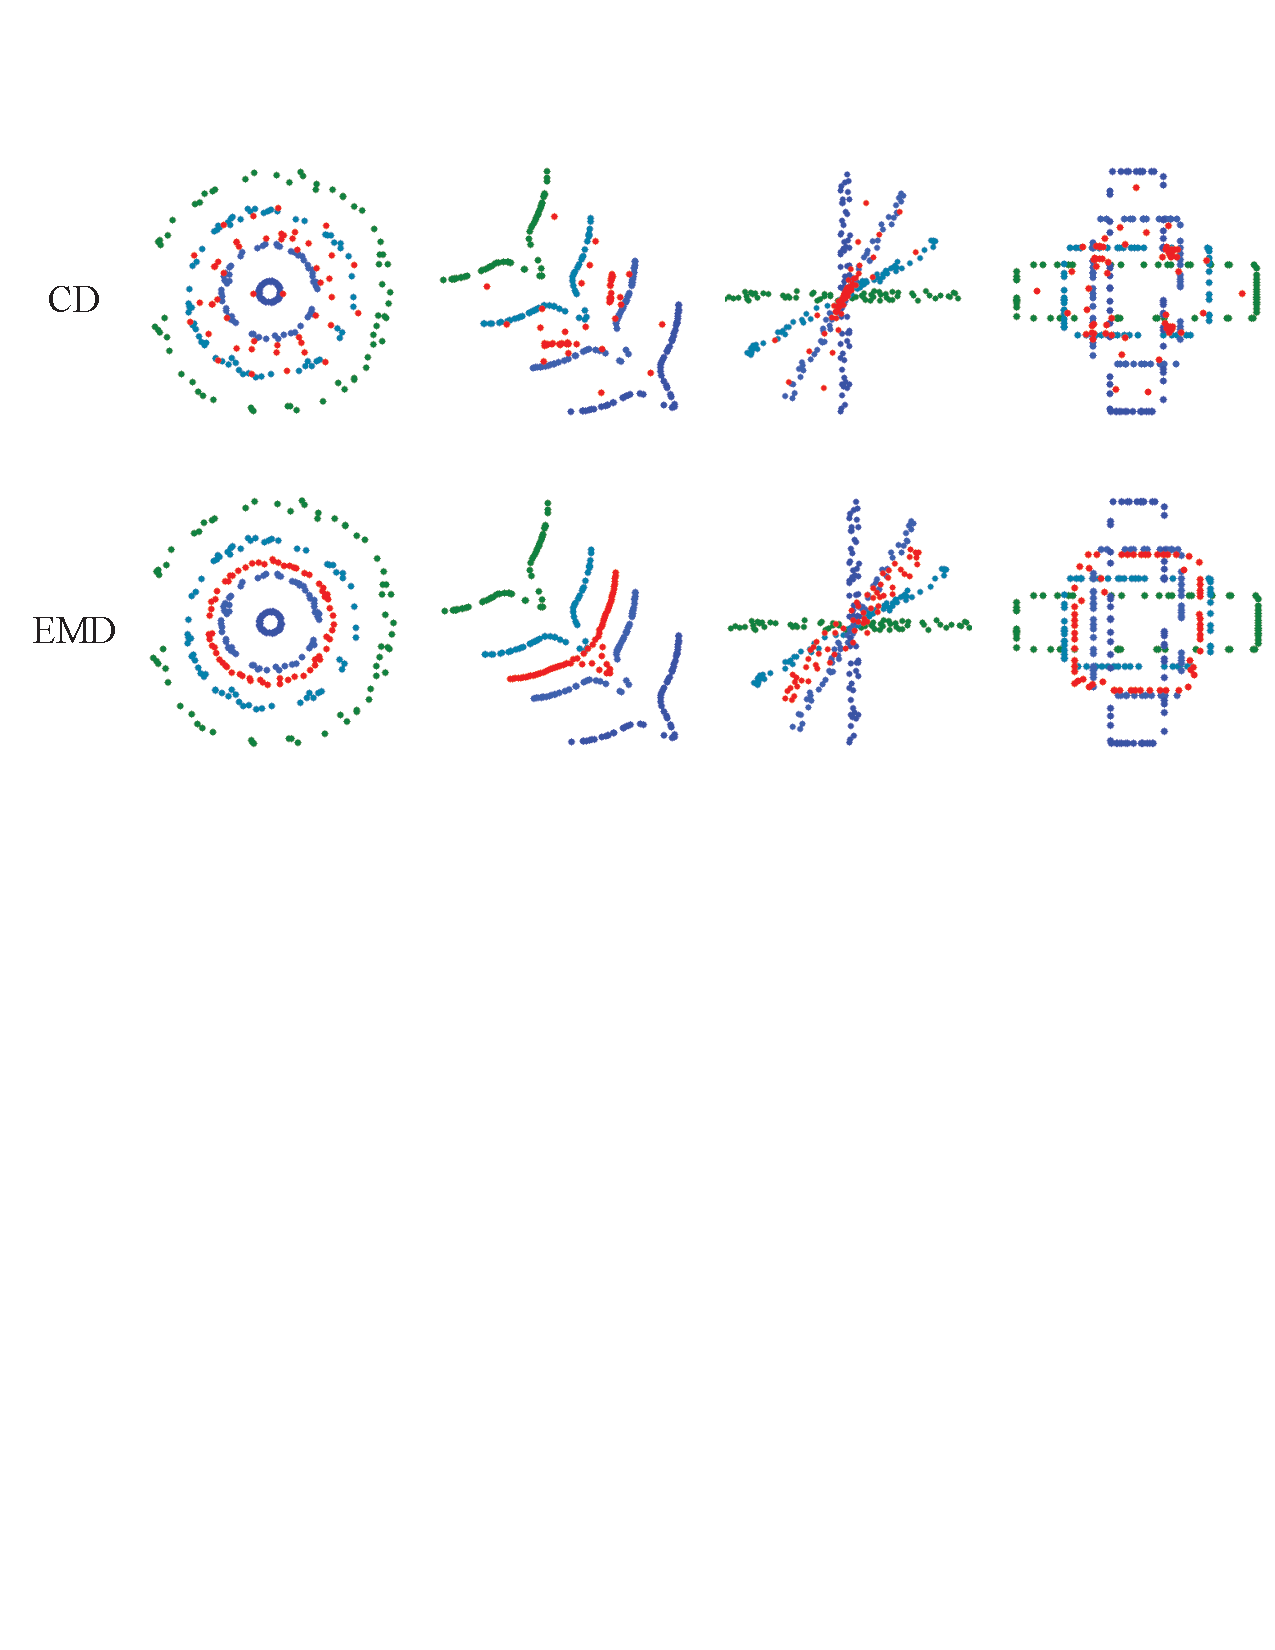
\includegraphics[width=\linewidth]{./fig/interpolation}
  %\caption{The interpolation of point sets by Chamfer distance (CD) versus Earth %Mover's distance (EMD). Each column corresponds to one type of shape. For each %type, we compute the mean shape $E$ (red) from four samples $S_i$ with different %parameters (from green to blue), e.g., radius of a circle. The mean shape is %computed by solving the optimization problem $\min_E \sum_{i=1}^4 d^2(E, S_i)$, %where $d$ can be CD or EMD. We observe that the mean shape from EMD looks more %natural.}
  %\label{fig:interoplation}
%\end{figure}

\paragraph{Shape space}
Despite remarkable expressive power embedded in the deep layers, neural networks inevitably encounter uncertainty in predicting the precise geometry of an object. Such uncertainty could arise from limited network capacity, insufficient use of input resolution, or the ambiguity of groundtruth due to information loss in 3D-2D projection. Facing the inherent inability to resolve the shape precisely, neural networks tend to predict a ``mean'' shape averaging out the space of uncertainty. The mean shape carries the characteristics of the distance itself.

In Figure~\ref{fig:mean}, we illustrate the distinct mean-shape behavior of EMD and CD on synthetic shape distributions, by minimizing
% \begin{equation*}
% \begin{aligned}
% \underset{x}{\mbox{minimize}}&&\mathrm{E}_{s\sim S}[L(x,s)]
% \end{aligned}
% \end{equation*}
$\mathrm{E}_{s\sim \mathbb{S}}[L(x,s)]$
through stochastic gradient descent, where $\mathbb{S}$ is a given shape distribution, $L$ is one of the distance functions. 

In the first and the second case, there is a single continuously changing hidden variable, namely the radius of the circle in (a) and the location of the arc in (b). EMD roughly captures the shape corresponding to the mean value of the hidden variable. In contrast CD induces a splashy shape that blurs the shape's geometric structure. In the latter two cases, there are categorical hidden variables: which corner the square is located at (c) and whether there is a circle besides the bar (d). To address the uncertain presence of the varying part, the minimizer of CD distributes some points outside the main body at the correct locations; while the minimizer of EMD is considerably distorted.

\begin{figure}[t!]
\centering
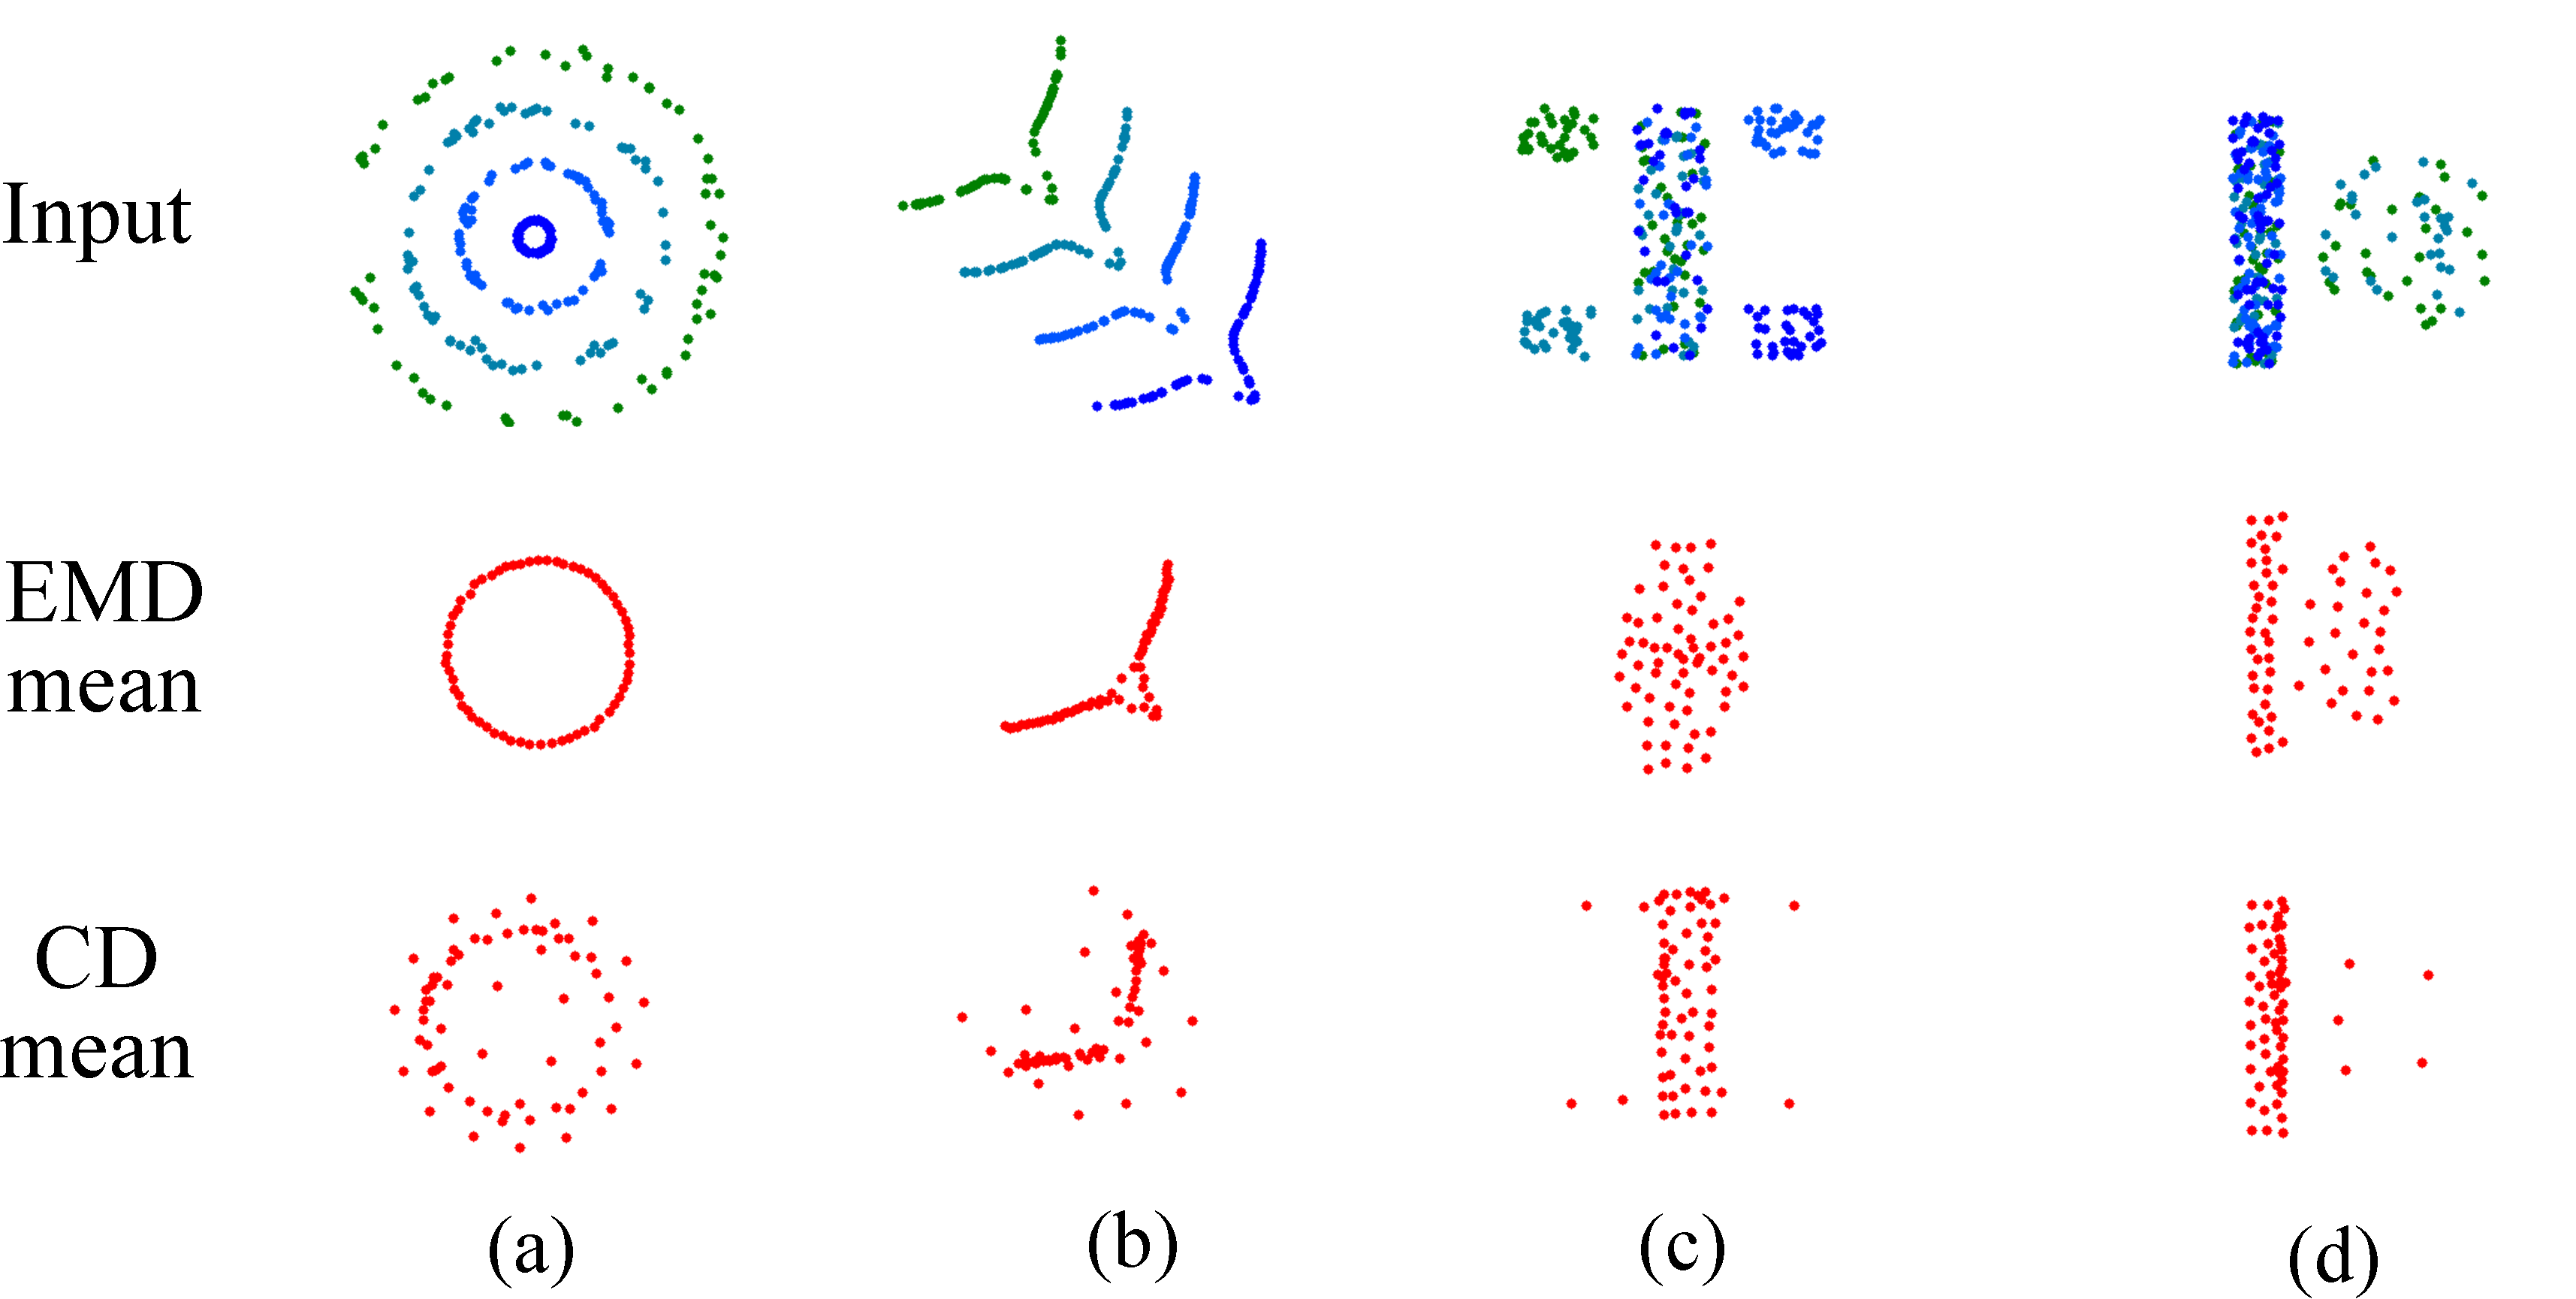
\includegraphics[width=0.9\linewidth]{./fig/show_mean.pdf}
\caption{Mean-shape behavior of EMD and CD. The shape distributions are (a) a circle with varying radius; (b) a spiky arc moving along the diagonal; (c) a rectangle bar, with a square-shaped attachment allocated randomly on one of the four corners; (d) a bar, with a circular disk appearing next to it with probability 0.5. The red dots plot the mean shape calculated according to EMD and CD accordingly.}
\label{fig:mean}
\end{figure}

\subsection{Generation of Multiple Plausible Shapes}
\label{sec:method:gan}
% \todo{
% this is an inherent property of our problem. give an illustrative example to convince the reader.
% 
% therefore, ideally, we should be able to generate the space of plausible shapes. we can think that the gt for each training data is just a sample from the groundtruth space. 
% 
% so we come up with the idea -- make multiple predictions, and at least one of the prediction should match the groundtruth.
% }

Our problem solves an ill-posed problem of 3D structural recovery from a single projection. Posed as a regression problem, ambiguity of the prediction arises at test time -- the depth for visible parts is under-determined, and the geometry for invisible parts has to be hallucinated by guessing. In a statistical view, reasonable predictions from the input image form a distribution.  Reflected in the training set, two images that look alike may have rather different groundtruth shapes. Recall the discussion in the previous section -- the ambiguity of groundtruth shape may significantly affect the trained predictor, as the loss function \eqref{eqn:loss} induces our model to predict the mean of possible shapes.  

\begin{figure}[t!]
  \centering
  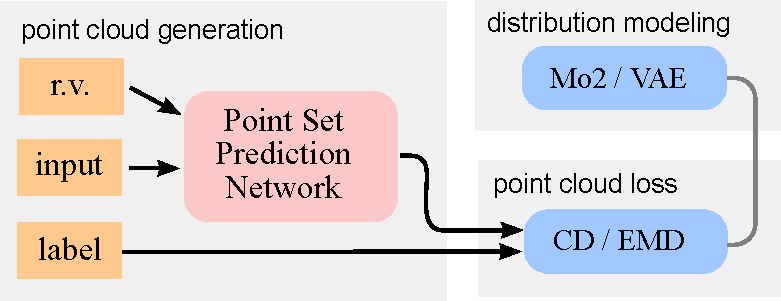
\includegraphics[width=0.8\linewidth]{./fig/system.pdf}
  \caption{System structure. By plugging in distributional modeling module, our system is capable of generating multiple predictions. }
  \label{fig:network}%xiao qiang zhen bang
\end{figure}
%ndeed, the nice interpolation ability of EMD helps us to generate a reasonable mean shape; however, ideally we should fully characterize the landscape of the groundtruth distribution, or be able to sample plausible candidates accordingly. Statistically, we are looking for a conditional sampler dependent on the input image. In this view, the groundtruth shape of each image provided by the training data is in fact a sample from the groundtruth distribution.

To better model the uncertainty or inherent ambiguity (e.g. unseen parts in the single view), we enable the system to generate distributional output. We expect that the random variable $r$ passed to $\mathbb{G}$ (see Eq~\eqref{eqn:main}) would help it explore the groundtruth distribution, in analogy to conditional GAN (CGAN)~\cite{mirza2014conditional}. However, naively plugging $\mathbb{G}$ from Eq~\eqref{eqn:main} into Loss~\eqref{eqn:loss} to predict $S_i^{pred}$ won't work, as the loss minimization will nullify the randomness. It is also unclear how to make CGAN work in our scenario, as building a discriminator that directly consumes a point set is itself an open problem. 

The problem can be solved by more complex frameworks like VAE, where we can incorporate secondary input channels (e.g. another view). However, we find practically a simple and effective method for uncertainty modeling: the MoN loss. We train our network by minimizing a loss function as below:
\begin{equation}
    \begin{aligned}
    \underset{\Theta}{\mbox{minimize}} 
    && 
    \sum_k 
        \min_{
            \substack{r_j\sim \mathbb{N}(\mathbf{0}, \mathbf{I})\\1\le j\le n}
        }
        \{
            d(\mathbb{G}(I_k, r_j;\Theta), S_k^{gt})
        \}
    \end{aligned} 
    \label{eqn:gan}
\end{equation}    

We explain the rationale behind Problem~\eqref{eqn:gan} here. Given an image $I_k$, $\mathbb{G}$ makes $n$ predictions by perturbing the input with $n$ random vectors $r_j$. Intuitively, we expect that one of the predictions will be close to the groundtruth $S_k^{gt}$ given by the training data, meaning that the minimum of the $n$ distances between each prediction and the groundtruth must be small. 

We name this loss as Min-of-N loss (MoN), since it comes from the minimum of $n$ distances. Any of the point set regression networks in Fig~\ref{fig:pointnet} can be plugged into the meta network in Fig~\ref{fig:network} incorporating the MoN loss. In practice, we find that setting $n=2$ already enables our method to well explore the groundtruth space.  Please refer to Sec~\ref{sec:exp:gan} for experiment results.

An alternative way to achieve the conditional shape sampler is by a conditional variational autoencoder. For more details about variational autoencoders, please refer to \cite{doersch2016tutorial}.  Fig~\ref{fig:VAE} shows the system architecture for training and testing a conditional variational autoencoder $P(S|X)$ in our case. Here, $X$ is the input image and $S$ is the \emph{point cloud} representation of the groundtruth 3D shape. At training time, each input image $X$ will be augmented by a random variable that is conditioned on $Y$, which takes the \emph{volumetric} representation of the groundtruth shape $S$. A 3D convolutional network is used as the encoder $Q$ (see \cite{maturana2015voxnet} for a good reference of 3D conv networks). Therefore, a local proximity in the embedding space contains the variations of possible groundtruth 3D shapes.

\begin{figure}
\centering
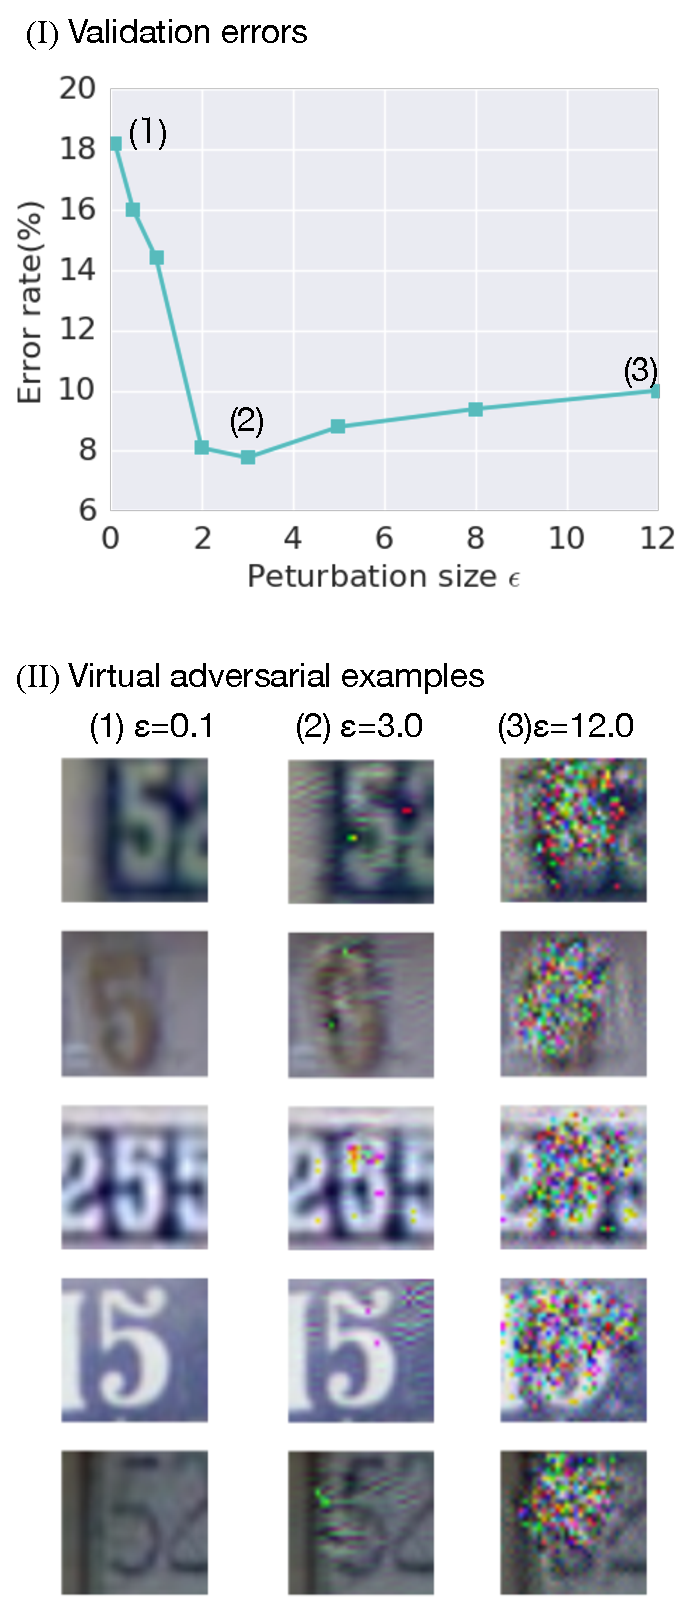
\includegraphics[width=\linewidth]{./fig/vae.pdf}
\caption{Network for conditional variational autoencoder shape sampler $P(S|X)$. Left: a training-time conditional variational autoencoder implemented as a feedforward neural network. Here, $Y$ is the volumetric form of the groundtruth shape $S$, whereas $f(z, X)$ is the point cloud form of the predicted shape for $S$. Right: the same model at test time. (Modified from Doersch et al.~\cite{doersch2016tutorial})}
\label{fig:VAE}
\end{figure}

% An alternative way to build the conditional sampler is through conditional variational autoencoder (VAE) technique, which requires a few additional modules. We explain the VAE version in the supplementary. 





\section{Experiments}
\label{sect:experiments}

% \begin{figure*}
%   \centering
%   \setlength{\tabcolsep}{0pt}
%   \setlength\figurewidth{0.05\textwidth}
%   \newcommand{\example}[1]{\raisebox{-.4\height}{\includegraphics[width=\figurewidth]{./figures/domains_examples/#1}}}
%   \begin{sc}
%   \begin{tabular}{r@{\hskip 1cm} ccccccccccc}
%     MNIST \cite{LeCun98} &
%     \example{mnist_0.png} &
%     \example{mnist_1.png} &
%     \example{mnist_2.png} &
%     \example{mnist_3.png} &
%     \example{mnist_4.png} &
%     \example{mnist_5.png} &
%     \example{mnist_6.png} &
%     \example{mnist_7.png} &
%     \example{mnist_8.png} &
%     \example{mnist_9.png} &
%     \example{mnist_10.png}\\
%     MNIST ($ | \Delta | $, BG) &
%     \example{mnisti_0.png} &
%     \example{mnisti_1.png} &
%     \example{mnisti_2.png} &
%     \example{mnisti_3.png} &
%     \example{mnisti_4.png} &
%     \example{mnisti_5.png} &
%     \example{mnisti_6.png} &
%     \example{mnisti_7.png} &
%     \example{mnisti_8.png} &
%     \example{mnisti_9.png} &
%     \example{mnisti_10.png}\\
%     Syn Numbers &
%     \example{syn_0.png} &
%     \example{syn_1.png} &
%     \example{syn_2.png} &
%     \example{syn_3.png} &
%     \example{syn_4.png} &
%     \example{syn_5.png} &
%     \example{syn_6.png} &
%     \example{syn_7.png} &
%     \example{syn_8.png} &
%     \example{syn_9.png} &
%     \example{syn_10.png}\\
%     SVHN \cite{Netzer11} &
%     \example{svhn_0.png} &
%     \example{svhn_1.png} &
%     \example{svhn_2.png} &
%     \example{svhn_3.png} &
%     \example{svhn_4.png} &
%     \example{svhn_5.png} &
%     \example{svhn_6.png} &
%     \example{svhn_7.png} &
%     \example{svhn_8.png} &
%     \example{svhn_9.png} &
%     \example{svhn_10.png}\\
%     Syn Signs &
%     \example{synsgn_11.png} &
%     \example{synsgn_1.png} &
%     \example{synsgn_2.png} &
%     \example{synsgn_3.png} &
%     \example{synsgn_4.png} &
%     \example{synsgn_5.png} &
%     \example{synsgn_12.png} &
%     \example{synsgn_7.png} &
%     \example{synsgn_8.png} &
%     \example{synsgn_9.png} &
%     \example{synsgn_10.png}\\
%     GTSRB \cite{Stallkamp12} &
%     \example{gtsrb_0.png} &
%     \example{gtsrb_1.png} &
%     \example{gtsrb_2.png} &
%     \example{gtsrb_3.png} &
%     \example{gtsrb_4.png} &
%     \example{gtsrb_5.png} &
%     \example{gtsrb_6.png} &
%     \example{gtsrb_7.png} &
%     \example{gtsrb_8.png} &
%     \example{gtsrb_9.png} &
%     \example{gtsrb_10.png}\\
%     % CIFAR-10 \cite{Krizhevsky09} &
%     % \example{cifar10_0.png} &
%     % \example{cifar10_1.png} &
%     % \example{cifar10_2.png} &
%     % \example{cifar10_3.png} &
%     % \example{cifar10_4.png} &
%     % \example{cifar10_5.png} &
%     % \example{cifar10_11.png} &
%     % \example{cifar10_7.png} &
%     % \example{cifar10_8.png} &
%     % \example{cifar10_9.png} &
%     % \example{cifar10_10.png}\\
%     % STL-10 \cite{Coates11} &
%     % \example{stl10_12.png} &
%     % \example{stl10_1.png} &
%     % \example{stl10_2.png} &
%     % \example{stl10_3.png} &
%     % \example{stl10_4.png} &
%     % \example{stl10_5.png} &
%     % \example{stl10_6.png} &
%     % \example{stl10_13.png} &
%     % \example{stl10_8.png} &
%     % \example{stl10_9.png} &
%     % \example{stl10_10.png}\\
%   \end{tabular}
%   \end{sc}
%   \vskip 2.5mm
%   \caption{\todo[What to do with this figure? Add Office? Remove?]Random samples from the datasets used in the experiments. See \sect{exper_quant} for details.}
%   \label{fig:exper_domains_examples}
% \end{figure*}

\begin{figure*}
  \centering
  \setlength{\tabcolsep}{0pt}
  \setlength\figurewidth{0.05\textwidth}
  \newcommand{\example}[1]{\raisebox{-.4\height}{\includegraphics[width=\figurewidth]{./figures/domains_examples/#1}}}
  \begin{sc}
  \begin{small}
  \begin{tabular}{r@{\hskip 0.5cm} ccc c@{\hskip 0.4cm} ccc c@{\hskip 0.4cm} ccc c@{\hskip 0.4cm} ccc}
    &
    \multicolumn{3}{c}{MNIST} & &
    \multicolumn{3}{c}{Syn Numbers} & &
    \multicolumn{3}{c}{SVHN} & &
    \multicolumn{3}{c}{Syn Signs}\\
    
    Source &
    \example{mnist_0.png} &
    \example{mnist_1.png} &
    \example{mnist_3.png} & &
    
    \example{syn_0.png} &
    \example{syn_1.png} &
    \example{syn_2.png} & &
    
    \example{svhn_3.png} &
    \example{svhn_4.png} &
    \example{svhn_5.png} & &
    
    \example{synsgn_3.png} &
    \example{synsgn_4.png} &
    \example{synsgn_5.png}\\
    
    Target &
    \example{mnisti_0.png} &
    \example{mnisti_1.png} &
    \example{mnisti_2.png} & &
    
    \example{svhn_0.png} &
    \example{svhn_1.png} &
    \example{svhn_2.png} & &
    
    \example{mnist_4.png} &
    \example{mnist_5.png} &
    \example{mnist_6.png} & &
    
    \example{gtsrb_2.png} &
    \example{gtsrb_3.png} &
    \example{gtsrb_4.png}\\
    
    &
    \multicolumn{3}{c}{\rule{0pt}{0.35cm} MNIST-M} & &
    \multicolumn{3}{c}{SVHN} & &
    \multicolumn{3}{c}{MNIST} & &
    \multicolumn{3}{c}{GTSRB}\\
  \end{tabular}
  \end{small}
  \end{sc}
  \caption{Examples of domain pairs used in the experiments. See \sect{exper_quant} for details.}
  \label{fig:exper_domains_examples}
\end{figure*}


\begin{table*}[t]
  \vskip 0.15in
  \begin{center}
    \begin{small}
      \begin{sc}
        \renewcommand{\arraystretch}{1.5}
        \begin{tabular}{l r | c c c c}
          \hline
          \multirow{2}{*}{Method} & {\scriptsize Source} & MNIST & Syn Numbers & SVHN & Syn Signs \\
          & {\scriptsize Target} & MNIST-M & SVHN & MNIST & GTSRB \\
          \hline
          \multicolumn{2}{l |}{Source only} & 
          $ .5749 $                      & $ .8665 $                      & $ .5919 $                      & $ .7400 $                      \\
          \multicolumn{2}{l |}{SA \cite{Fernando13}} & 
          $ .6078 \; (7.9\%) $           & $ .8672 \; (1.3\%) $           & $ .6157 \; (5.9\%) $           & $ .7635 \; (9.1\%) $           \\
          \multicolumn{2}{l |}{Proposed approach} & 
          $ \mathbf{.8149} \; (57.9\%) $ & $ \mathbf{.9048} \; (66.1\%) $ & $ \mathbf{.7107} \; (29.3\%) $ & $ \mathbf{.8866} \; (56.7\%) $ \\
          \multicolumn{2}{l |}{Train on target} & 
          $ .9891 $                      & $ .9244 $                      & $ .9951 $                      & $ .9987 $                      \\
          \hline
        \end{tabular}
      \end{sc}
    \end{small}
  \end{center}
    \caption{Classification accuracies for digit image classifications for different source and target domains. {\sc MNIST-M} corresponds to difference-blended digits over non-uniform background. The first row corresponds to the lower performance bound (i.e.\ if no adaptation is performed). The last row corresponds to training on the target domain data with known class labels (upper bound on the DA performance). For each of the two DA methods (ours and \cite{Fernando13}) we show how much of the gap between the lower and the upper bounds was covered (in brackets). For all five cases, our approach outperforms \cite{Fernando13} considerably, and covers a big portion of the gap.\vspace{-0mm} }
  \label{tab:results}
  \vskip -0.1in
\end{table*}

\begin{table*}[t]
  \vskip 0.15in
  \begin{center}
    \begin{small}
      \begin{sc}
        \renewcommand{\arraystretch}{1.5}
        \begin{tabular}{l r | c c c}
          \hline
          \multirow{2}{*}{Method} & {\scriptsize Source} & Amazon & DSLR & Webcam \\
          & {\scriptsize Target} & Webcam & Webcam & DSLR \\
          \hline
          \multicolumn{2}{l |}{GFK(PLS, PCA) \cite{Gong12}} & 
          $ .464 \pm .005 $ & $ .613 \pm .004 $ & $ .663 \pm .004 $\\ 
          \multicolumn{2}{l |}{SA \cite{Fernando13}} & 
          $ .450 $ & $ .648 $ & $ .699 $\\ 
          \multicolumn{2}{l |}{DA-NBNN \cite{Tommasi13}} & 
          $ .528 \pm .037 $ & $ .766 \pm .017 $ & $ .762 \pm .025 $\\ 
          \multicolumn{2}{l |}{DLID \cite{Chopra13}} & 
          $ .519 $ & $ .782 $ & $ .899 $\\
          \multicolumn{2}{l |}{DeCAF$_6$ Source Only \cite{Donahue14}} &
          $ .522 \pm .017 $ & $ .915 \pm .015 $ & --\\ 
          \multicolumn{2}{l |}{DaNN \cite{Ghifary14}} & 
          $ .536 \pm .002 $ & $ .712 \pm .000 $ & $ .835 \pm .000 $\\ 
          \multicolumn{2}{l |}{DDC \cite{Tzeng14}} & 
          $ .594 \pm .008 $ & $ .925 \pm .003 $ & $ .917 \pm .008 $\\ 
          \multicolumn{2}{l |}{Proposed Approach} & 
          $ \mathbf{ .673 \pm .017 } $ & $ \mathbf{ .940 \pm .008 } $ & $ \mathbf{ .937 \pm .010 } $\\
          \hline
        \end{tabular}
      \end{sc}
    \end{small}
  \end{center}
    \caption{Accuracy evaluation of different DA approaches on the standard {\sc Office} \cite{Saenko10} dataset. Our method (last row) outperforms competitors setting the new state-of-the-art.}
  \label{tab:results_office}
\end{table*}

% Other rows refer to the following algorithms (from top to bottom): Geodesic Flow Kernel \cite{Gong12}, Subspace Alignment \cite{Fernando13}, Naive Bayes Nearest Neighbor \cite{Tommasi13},  deep learning approach from \cite{Chopra13}, DeCAF$_6$-features described in \cite{Donahue14}, Domain Adaptive NNs \cite{Ghifary14}, Deep Domain Confusion \cite{Tzeng14}.

\def\X{{\mathbf X}}
\def\y{{\mathbf y}}

% \vspace{2mm}\noindent {\bf Datasets.}
% \label{sect:exper_datasets}

% In order to test our method in the setting of traffic signs classification we obtained~100,000 synthetic images ({\sc Syn~Signs}) simulating various photoshooting conditions. This dataset was used in conjunction with {\it The German Traffic Sign Recognition Benchmark} ({\sc GTSRB}) \cite{Stallkamp12}.

% Finally, we perform domain adaption for the {\sc CIFAR-10} and the {\sc STL-10} downsampled to the size of $ 32 \times 32 $. This pair is considerably different from the previously mentioned datasets as the intra-class variability here is higher.

We perform extensive evaluation of the proposed approach on a number of popular image datasets and their modifications. These include large-scale datasets of small images popular with deep learning methods, and the {\sc Office} datasets \cite{Saenko10}, which are a {\em de facto} standard for domain adaptation in computer vision, but have much fewer images.

\vspace{2mm}\noindent {\bf Baselines.} For the bulk of experiments the following baselines are evaluated. The \textbf{source-only} model is trained without consideration for target-domain data (no domain classifier branch included into the network). The \textbf{train-on-target} model is trained on the target domain with class labels revealed. This model serves as an upper bound on DA methods, assuming that target data are abundant and the shift between the domains is considerable. 

In addition, we compare our approach against the recently proposed unsupervised DA method based on \textbf{subspace alignment (SA)} \cite{Fernando13}, which is simple to setup and test on new datasets, but has also been shown to perform very well in experimental comparisons with other ``shallow'' DA methods. To boost the performance of this baseline, we pick its most important free parameter (the number of principal components) from the range $ \{ 2, \ldots, 60 \} $, so that the test performance on the target domain is maximized. To apply SA in our setting, we train a source-only model and then consider the activations of the last hidden layer in the label predictor (before the final linear classifier) as descriptors/features, and learn the mapping between the source and the target domains \cite{Fernando13}.

Since the SA baseline requires to train a new classifier after adapting the features, and in order to put all the compared settings on an equal footing, we retrain the last layer of the label predictor using a standard linear SVM~\cite{liblinear} for all four considered methods (including ours; the performance on the target domain remains approximately the same after the retraining). 

For the {\sc Office} dataset \cite{Saenko10}, we directly compare the performance of our full network (feature extractor and label predictor) against recent DA approaches using previously published results.

\vspace{2mm}\noindent {\bf CNN architectures.} In general, we compose feature extractor from two or three convolutional layers, picking their exact configurations from previous works. We give the exact architectures in \ref{sect:appendix_archs}.

For the domain adaptator we stick to the three fully connected layers ($x\rightarrow1024\rightarrow1024\rightarrow2$), except for {\sc MNIST} where we used a simpler ($x\rightarrow100\rightarrow2$) architecture to speed up the experiments.

For loss functions, we set $ L_y $ and $ L_d $ to be the logistic regression loss and the binomial cross-entropy respectively.

\vspace{2mm}\noindent {\bf CNN training procedure.}
The model is trained on $128$-sized batches. Images are preprocessed by the mean subtraction. A half of each batch is populated by the samples from the source domain (with known labels), the rest is comprised of the target domain (with unknown labels).

In order to suppress noisy signal from the domain classifier at the early stages of the training procedure instead of fixing the adaptation factor $ \lambda $, we gradually change it from $0$ to $1$ using the following schedule:
\begin{equation}
  \lambda_p = \frac{2}{1 + \exp(-\gamma \cdot p)} - 1,
\end{equation}
where $\gamma$ was set to $10$ in all experiments (the schedule was not optimized/tweaked). Further details on the CNN training can be found in \ref{sect:appendix_training}.

\vspace{2mm}\noindent {\bf Visualizations.}
We use t-SNE \cite{Maaten13} projection to visualize feature distributions at different points of the network, while color-coding the domains (\fig{exper_adapt_vis}). We observe strong correspondence between the success of the adaptation in terms of the classification accuracy for the target domain, and the overlap between the domain distributions in such visualizations.
 
\vspace{2mm}\noindent {\bf Choosing meta-parameters.} 
In general, good unsupervised DA methods should provide ways to set meta-parameters (such as $\lambda$, the learning rate, the momentum rate, the network architecture for our method) in an unsupervised way, i.e.\ without referring to labeled data in the target domain. %Here we would like to give few recommendations concerning this matter. First, as it was pointed out in \sect{theory} the domain classifier should not be significantly more complex than the label predictor. 
In our method, one can assess the performance of the whole system (and the effect of changing hyper-parameters) by observing the test error on the source domain {\em and} the domain classifier error. In general, we observed a good correspondence between the success of adaptation and these errors (adaptation is more successful when the source domain test error is low, while the domain classifier error is high).
In addition, the layer, where the the domain adaptator is attached can be picked by computing difference between means as suggested in \cite{Tzeng14}. 

% \begin{figure*}
%   \centering
%   {\sc MNIST $ \rightarrow $ MNIST ($ | \Delta | $, bg)}: top feature extractor layer
%   \setcounter{subfigure}{0}
%   \subfigure[Non-adapted]{%%
%     \scalebox{0.8}{%% Creator: Matplotlib, PGF backend
%%
%% To include the figure in your LaTeX document, write
%%   \input{<filename>.pgf}
%%
%% Make sure the required packages are loaded in your preamble
%%   \usepackage{pgf}
%%
%% Figures using additional raster images can only be included by \input if
%% they are in the same directory as the main LaTeX file. For loading figures
%% from other directories you can use the `import` package
%%   \usepackage{import}
%% and then include the figures with
%%   \import{<path to file>}{<filename>.pgf}
%%
%% Matplotlib used the following preamble
%%   \usepackage[utf8x]{inputenc}
%%   \usepackage[T1]{fontenc}
%%
\begingroup%
\makeatletter%
\begin{pgfpicture}%
\pgfpathrectangle{\pgfpointorigin}{\pgfqpoint{3.338520in}{2.040000in}}%
\pgfusepath{use as bounding box}%
\begin{pgfscope}%
\pgfsetbuttcap%
\pgfsetroundjoin%
\definecolor{currentfill}{rgb}{1.000000,1.000000,1.000000}%
\pgfsetfillcolor{currentfill}%
\pgfsetlinewidth{0.000000pt}%
\definecolor{currentstroke}{rgb}{1.000000,1.000000,1.000000}%
\pgfsetstrokecolor{currentstroke}%
\pgfsetdash{}{0pt}%
\pgfpathmoveto{\pgfqpoint{0.000000in}{-0.000000in}}%
\pgfpathlineto{\pgfqpoint{3.338520in}{-0.000000in}}%
\pgfpathlineto{\pgfqpoint{3.338520in}{2.040000in}}%
\pgfpathlineto{\pgfqpoint{0.000000in}{2.040000in}}%
\pgfpathclose%
\pgfusepath{fill}%
\end{pgfscope}%
\begin{pgfscope}%
\pgftext[at=\pgfqpoint{0.510000in}{0.348333in},left,bottom]{\pgfimage[interpolate=true,width=2.553333in,height=1.500000in]{./figures/adaptation_vis/pool2_mnist2inv_before-img0.png}}%
\end{pgfscope}%
\begin{pgfscope}%
\pgftext[at=\pgfqpoint{0.805000in}{0.383333in},left,bottom]{\pgfimage[interpolate=true,width=2.201667in,height=1.371667in]{./figures/adaptation_vis/pool2_mnist2inv_before-img1.png}}%
\end{pgfscope}%
\end{pgfpicture}%
\makeatother%
\endgroup%
}}%%
%   \subfigure[Adapted]{%%
%     \scalebox{0.8}{%% Creator: Matplotlib, PGF backend
%%
%% To include the figure in your LaTeX document, write
%%   \input{<filename>.pgf}
%%
%% Make sure the required packages are loaded in your preamble
%%   \usepackage{pgf}
%%
%% Figures using additional raster images can only be included by \input if
%% they are in the same directory as the main LaTeX file. For loading figures
%% from other directories you can use the `import` package
%%   \usepackage{import}
%% and then include the figures with
%%   \import{<path to file>}{<filename>.pgf}
%%
%% Matplotlib used the following preamble
%%   \usepackage[utf8x]{inputenc}
%%   \usepackage[T1]{fontenc}
%%
\begingroup%
\makeatletter%
\begin{pgfpicture}%
\pgfpathrectangle{\pgfpointorigin}{\pgfqpoint{3.340000in}{2.040000in}}%
\pgfusepath{use as bounding box}%
\begin{pgfscope}%
\pgfsetbuttcap%
\pgfsetroundjoin%
\definecolor{currentfill}{rgb}{1.000000,1.000000,1.000000}%
\pgfsetfillcolor{currentfill}%
\pgfsetlinewidth{0.000000pt}%
\definecolor{currentstroke}{rgb}{1.000000,1.000000,1.000000}%
\pgfsetstrokecolor{currentstroke}%
\pgfsetdash{}{0pt}%
\pgfpathmoveto{\pgfqpoint{0.000000in}{-0.000000in}}%
\pgfpathlineto{\pgfqpoint{3.340000in}{-0.000000in}}%
\pgfpathlineto{\pgfqpoint{3.340000in}{2.040000in}}%
\pgfpathlineto{\pgfqpoint{0.000000in}{2.040000in}}%
\pgfpathclose%
\pgfusepath{fill}%
\end{pgfscope}%
\begin{pgfscope}%
\pgftext[at=\pgfqpoint{0.518333in}{0.321667in},left,bottom]{\pgfimage[interpolate=true,width=2.565000in,height=1.550000in]{./figures/adaptation_vis/pool2_mnist2inv_after-img0.png}}%
\end{pgfscope}%
\begin{pgfscope}%
\pgftext[at=\pgfqpoint{0.518333in}{0.321667in},left,bottom]{\pgfimage[interpolate=true,width=2.565000in,height=1.553333in]{./figures/adaptation_vis/pool2_mnist2inv_after-img1.png}}%
\end{pgfscope}%
\end{pgfpicture}%
\makeatother%
\endgroup%
}}\\
%   \vspace{5mm}
%   {\sc Syn Numbers $ \rightarrow $ SVHN}: last hidden layer of the label predictor
%   \setcounter{subfigure}{0}
%   \subfigure[Non-adapted]{%%
%     \scalebox{0.8}{%% Creator: Matplotlib, PGF backend
%%
%% To include the figure in your LaTeX document, write
%%   \input{<filename>.pgf}
%%
%% Make sure the required packages are loaded in your preamble
%%   \usepackage{pgf}
%%
%% Figures using additional raster images can only be included by \input if
%% they are in the same directory as the main LaTeX file. For loading figures
%% from other directories you can use the `import` package
%%   \usepackage{import}
%% and then include the figures with
%%   \import{<path to file>}{<filename>.pgf}
%%
%% Matplotlib used the following preamble
%%   \usepackage[utf8x]{inputenc}
%%   \usepackage[T1]{fontenc}
%%
\begingroup%
\makeatletter%
\begin{pgfpicture}%
\pgfpathrectangle{\pgfpointorigin}{\pgfqpoint{3.340000in}{2.040000in}}%
\pgfusepath{use as bounding box}%
\begin{pgfscope}%
\pgfsetbuttcap%
\pgfsetroundjoin%
\definecolor{currentfill}{rgb}{1.000000,1.000000,1.000000}%
\pgfsetfillcolor{currentfill}%
\pgfsetlinewidth{0.000000pt}%
\definecolor{currentstroke}{rgb}{1.000000,1.000000,1.000000}%
\pgfsetstrokecolor{currentstroke}%
\pgfsetdash{}{0pt}%
\pgfpathmoveto{\pgfqpoint{0.000000in}{-0.000000in}}%
\pgfpathlineto{\pgfqpoint{3.340000in}{-0.000000in}}%
\pgfpathlineto{\pgfqpoint{3.340000in}{2.040000in}}%
\pgfpathlineto{\pgfqpoint{0.000000in}{2.040000in}}%
\pgfpathclose%
\pgfusepath{fill}%
\end{pgfscope}%
\begin{pgfscope}%
\pgftext[at=\pgfqpoint{0.491667in}{0.335000in},left,bottom]{\pgfimage[interpolate=true,width=2.618333in,height=1.531667in]{./figures/adaptation_vis/before-img0.png}}%
\end{pgfscope}%
\begin{pgfscope}%
\pgftext[at=\pgfqpoint{0.758333in}{0.331667in},left,bottom]{\pgfimage[interpolate=true,width=2.171667in,height=1.436667in]{./figures/adaptation_vis/before-img1.png}}%
\end{pgfscope}%
\begin{pgfscope}%
\pgfsetbuttcap%
\pgfsetroundjoin%
\definecolor{currentfill}{rgb}{0.000000,0.000000,1.000000}%
\pgfsetfillcolor{currentfill}%
\pgfsetfillopacity{0.300000}%
\pgfsetlinewidth{0.150562pt}%
\definecolor{currentstroke}{rgb}{0.000000,0.000000,0.000000}%
\pgfsetstrokecolor{currentstroke}%
\pgfsetstrokeopacity{0.300000}%
\pgfsetdash{}{0pt}%
\pgfpathmoveto{\pgfqpoint{2.521160in}{1.775861in}}%
\pgfpathcurveto{\pgfqpoint{2.525278in}{1.775861in}}{\pgfqpoint{2.529228in}{1.777497in}}{\pgfqpoint{2.532140in}{1.780409in}}%
\pgfpathcurveto{\pgfqpoint{2.535052in}{1.783321in}}{\pgfqpoint{2.536688in}{1.787271in}}{\pgfqpoint{2.536688in}{1.791389in}}%
\pgfpathcurveto{\pgfqpoint{2.536688in}{1.795507in}}{\pgfqpoint{2.535052in}{1.799457in}}{\pgfqpoint{2.532140in}{1.802369in}}%
\pgfpathcurveto{\pgfqpoint{2.529228in}{1.805281in}}{\pgfqpoint{2.525278in}{1.806917in}}{\pgfqpoint{2.521160in}{1.806917in}}%
\pgfpathcurveto{\pgfqpoint{2.517042in}{1.806917in}}{\pgfqpoint{2.513092in}{1.805281in}}{\pgfqpoint{2.510180in}{1.802369in}}%
\pgfpathcurveto{\pgfqpoint{2.507268in}{1.799457in}}{\pgfqpoint{2.505631in}{1.795507in}}{\pgfqpoint{2.505631in}{1.791389in}}%
\pgfpathcurveto{\pgfqpoint{2.505631in}{1.787271in}}{\pgfqpoint{2.507268in}{1.783321in}}{\pgfqpoint{2.510180in}{1.780409in}}%
\pgfpathcurveto{\pgfqpoint{2.513092in}{1.777497in}}{\pgfqpoint{2.517042in}{1.775861in}}{\pgfqpoint{2.521160in}{1.775861in}}%
\pgfpathclose%
\pgfusepath{stroke,fill}%
\end{pgfscope}%
\begin{pgfscope}%
\pgfsetbuttcap%
\pgfsetroundjoin%
\definecolor{currentfill}{rgb}{0.000000,0.000000,1.000000}%
\pgfsetfillcolor{currentfill}%
\pgfsetfillopacity{0.300000}%
\pgfsetlinewidth{0.150562pt}%
\definecolor{currentstroke}{rgb}{0.000000,0.000000,0.000000}%
\pgfsetstrokecolor{currentstroke}%
\pgfsetstrokeopacity{0.300000}%
\pgfsetdash{}{0pt}%
\pgfpathmoveto{\pgfqpoint{2.598938in}{1.785583in}}%
\pgfpathcurveto{\pgfqpoint{2.603056in}{1.785583in}}{\pgfqpoint{2.607006in}{1.787219in}}{\pgfqpoint{2.609918in}{1.790131in}}%
\pgfpathcurveto{\pgfqpoint{2.612830in}{1.793043in}}{\pgfqpoint{2.614466in}{1.796993in}}{\pgfqpoint{2.614466in}{1.801111in}}%
\pgfpathcurveto{\pgfqpoint{2.614466in}{1.805229in}}{\pgfqpoint{2.612830in}{1.809179in}}{\pgfqpoint{2.609918in}{1.812091in}}%
\pgfpathcurveto{\pgfqpoint{2.607006in}{1.815003in}}{\pgfqpoint{2.603056in}{1.816639in}}{\pgfqpoint{2.598938in}{1.816639in}}%
\pgfpathcurveto{\pgfqpoint{2.594819in}{1.816639in}}{\pgfqpoint{2.590869in}{1.815003in}}{\pgfqpoint{2.587957in}{1.812091in}}%
\pgfpathcurveto{\pgfqpoint{2.585045in}{1.809179in}}{\pgfqpoint{2.583409in}{1.805229in}}{\pgfqpoint{2.583409in}{1.801111in}}%
\pgfpathcurveto{\pgfqpoint{2.583409in}{1.796993in}}{\pgfqpoint{2.585045in}{1.793043in}}{\pgfqpoint{2.587957in}{1.790131in}}%
\pgfpathcurveto{\pgfqpoint{2.590869in}{1.787219in}}{\pgfqpoint{2.594819in}{1.785583in}}{\pgfqpoint{2.598938in}{1.785583in}}%
\pgfpathclose%
\pgfusepath{stroke,fill}%
\end{pgfscope}%
\begin{pgfscope}%
\pgfsetbuttcap%
\pgfsetroundjoin%
\definecolor{currentfill}{rgb}{0.000000,0.000000,1.000000}%
\pgfsetfillcolor{currentfill}%
\pgfsetfillopacity{0.300000}%
\pgfsetlinewidth{0.150562pt}%
\definecolor{currentstroke}{rgb}{0.000000,0.000000,0.000000}%
\pgfsetstrokecolor{currentstroke}%
\pgfsetstrokeopacity{0.300000}%
\pgfsetdash{}{0pt}%
\pgfpathmoveto{\pgfqpoint{2.676715in}{1.771000in}}%
\pgfpathcurveto{\pgfqpoint{2.680833in}{1.771000in}}{\pgfqpoint{2.684783in}{1.772636in}}{\pgfqpoint{2.687695in}{1.775548in}}%
\pgfpathcurveto{\pgfqpoint{2.690607in}{1.778460in}}{\pgfqpoint{2.692244in}{1.782410in}}{\pgfqpoint{2.692244in}{1.786528in}}%
\pgfpathcurveto{\pgfqpoint{2.692244in}{1.790646in}}{\pgfqpoint{2.690607in}{1.794596in}}{\pgfqpoint{2.687695in}{1.797508in}}%
\pgfpathcurveto{\pgfqpoint{2.684783in}{1.800420in}}{\pgfqpoint{2.680833in}{1.802056in}}{\pgfqpoint{2.676715in}{1.802056in}}%
\pgfpathcurveto{\pgfqpoint{2.672597in}{1.802056in}}{\pgfqpoint{2.668647in}{1.800420in}}{\pgfqpoint{2.665735in}{1.797508in}}%
\pgfpathcurveto{\pgfqpoint{2.662823in}{1.794596in}}{\pgfqpoint{2.661187in}{1.790646in}}{\pgfqpoint{2.661187in}{1.786528in}}%
\pgfpathcurveto{\pgfqpoint{2.661187in}{1.782410in}}{\pgfqpoint{2.662823in}{1.778460in}}{\pgfqpoint{2.665735in}{1.775548in}}%
\pgfpathcurveto{\pgfqpoint{2.668647in}{1.772636in}}{\pgfqpoint{2.672597in}{1.771000in}}{\pgfqpoint{2.676715in}{1.771000in}}%
\pgfpathclose%
\pgfusepath{stroke,fill}%
\end{pgfscope}%
\begin{pgfscope}%
\pgftext[x=2.798938in,y=1.762222in,left,base]{{\rmfamily\fontsize{8.000000}{9.600000}\selectfont Source}}%
\end{pgfscope}%
\begin{pgfscope}%
\pgfsetbuttcap%
\pgfsetroundjoin%
\definecolor{currentfill}{rgb}{1.000000,0.000000,0.000000}%
\pgfsetfillcolor{currentfill}%
\pgfsetfillopacity{0.300000}%
\pgfsetlinewidth{0.150562pt}%
\definecolor{currentstroke}{rgb}{0.000000,0.000000,0.000000}%
\pgfsetstrokecolor{currentstroke}%
\pgfsetstrokeopacity{0.300000}%
\pgfsetdash{}{0pt}%
\pgfpathmoveto{\pgfqpoint{2.521160in}{1.620928in}}%
\pgfpathcurveto{\pgfqpoint{2.525278in}{1.620928in}}{\pgfqpoint{2.529228in}{1.622564in}}{\pgfqpoint{2.532140in}{1.625476in}}%
\pgfpathcurveto{\pgfqpoint{2.535052in}{1.628388in}}{\pgfqpoint{2.536688in}{1.632338in}}{\pgfqpoint{2.536688in}{1.636456in}}%
\pgfpathcurveto{\pgfqpoint{2.536688in}{1.640574in}}{\pgfqpoint{2.535052in}{1.644524in}}{\pgfqpoint{2.532140in}{1.647436in}}%
\pgfpathcurveto{\pgfqpoint{2.529228in}{1.650348in}}{\pgfqpoint{2.525278in}{1.651984in}}{\pgfqpoint{2.521160in}{1.651984in}}%
\pgfpathcurveto{\pgfqpoint{2.517042in}{1.651984in}}{\pgfqpoint{2.513092in}{1.650348in}}{\pgfqpoint{2.510180in}{1.647436in}}%
\pgfpathcurveto{\pgfqpoint{2.507268in}{1.644524in}}{\pgfqpoint{2.505631in}{1.640574in}}{\pgfqpoint{2.505631in}{1.636456in}}%
\pgfpathcurveto{\pgfqpoint{2.505631in}{1.632338in}}{\pgfqpoint{2.507268in}{1.628388in}}{\pgfqpoint{2.510180in}{1.625476in}}%
\pgfpathcurveto{\pgfqpoint{2.513092in}{1.622564in}}{\pgfqpoint{2.517042in}{1.620928in}}{\pgfqpoint{2.521160in}{1.620928in}}%
\pgfpathclose%
\pgfusepath{stroke,fill}%
\end{pgfscope}%
\begin{pgfscope}%
\pgfsetbuttcap%
\pgfsetroundjoin%
\definecolor{currentfill}{rgb}{1.000000,0.000000,0.000000}%
\pgfsetfillcolor{currentfill}%
\pgfsetfillopacity{0.300000}%
\pgfsetlinewidth{0.150562pt}%
\definecolor{currentstroke}{rgb}{0.000000,0.000000,0.000000}%
\pgfsetstrokecolor{currentstroke}%
\pgfsetstrokeopacity{0.300000}%
\pgfsetdash{}{0pt}%
\pgfpathmoveto{\pgfqpoint{2.598938in}{1.630650in}}%
\pgfpathcurveto{\pgfqpoint{2.603056in}{1.630650in}}{\pgfqpoint{2.607006in}{1.632286in}}{\pgfqpoint{2.609918in}{1.635198in}}%
\pgfpathcurveto{\pgfqpoint{2.612830in}{1.638110in}}{\pgfqpoint{2.614466in}{1.642060in}}{\pgfqpoint{2.614466in}{1.646178in}}%
\pgfpathcurveto{\pgfqpoint{2.614466in}{1.650296in}}{\pgfqpoint{2.612830in}{1.654246in}}{\pgfqpoint{2.609918in}{1.657158in}}%
\pgfpathcurveto{\pgfqpoint{2.607006in}{1.660070in}}{\pgfqpoint{2.603056in}{1.661706in}}{\pgfqpoint{2.598938in}{1.661706in}}%
\pgfpathcurveto{\pgfqpoint{2.594819in}{1.661706in}}{\pgfqpoint{2.590869in}{1.660070in}}{\pgfqpoint{2.587957in}{1.657158in}}%
\pgfpathcurveto{\pgfqpoint{2.585045in}{1.654246in}}{\pgfqpoint{2.583409in}{1.650296in}}{\pgfqpoint{2.583409in}{1.646178in}}%
\pgfpathcurveto{\pgfqpoint{2.583409in}{1.642060in}}{\pgfqpoint{2.585045in}{1.638110in}}{\pgfqpoint{2.587957in}{1.635198in}}%
\pgfpathcurveto{\pgfqpoint{2.590869in}{1.632286in}}{\pgfqpoint{2.594819in}{1.630650in}}{\pgfqpoint{2.598938in}{1.630650in}}%
\pgfpathclose%
\pgfusepath{stroke,fill}%
\end{pgfscope}%
\begin{pgfscope}%
\pgfsetbuttcap%
\pgfsetroundjoin%
\definecolor{currentfill}{rgb}{1.000000,0.000000,0.000000}%
\pgfsetfillcolor{currentfill}%
\pgfsetfillopacity{0.300000}%
\pgfsetlinewidth{0.150562pt}%
\definecolor{currentstroke}{rgb}{0.000000,0.000000,0.000000}%
\pgfsetstrokecolor{currentstroke}%
\pgfsetstrokeopacity{0.300000}%
\pgfsetdash{}{0pt}%
\pgfpathmoveto{\pgfqpoint{2.676715in}{1.616066in}}%
\pgfpathcurveto{\pgfqpoint{2.680833in}{1.616066in}}{\pgfqpoint{2.684783in}{1.617703in}}{\pgfqpoint{2.687695in}{1.620615in}}%
\pgfpathcurveto{\pgfqpoint{2.690607in}{1.623527in}}{\pgfqpoint{2.692244in}{1.627477in}}{\pgfqpoint{2.692244in}{1.631595in}}%
\pgfpathcurveto{\pgfqpoint{2.692244in}{1.635713in}}{\pgfqpoint{2.690607in}{1.639663in}}{\pgfqpoint{2.687695in}{1.642575in}}%
\pgfpathcurveto{\pgfqpoint{2.684783in}{1.645487in}}{\pgfqpoint{2.680833in}{1.647123in}}{\pgfqpoint{2.676715in}{1.647123in}}%
\pgfpathcurveto{\pgfqpoint{2.672597in}{1.647123in}}{\pgfqpoint{2.668647in}{1.645487in}}{\pgfqpoint{2.665735in}{1.642575in}}%
\pgfpathcurveto{\pgfqpoint{2.662823in}{1.639663in}}{\pgfqpoint{2.661187in}{1.635713in}}{\pgfqpoint{2.661187in}{1.631595in}}%
\pgfpathcurveto{\pgfqpoint{2.661187in}{1.627477in}}{\pgfqpoint{2.662823in}{1.623527in}}{\pgfqpoint{2.665735in}{1.620615in}}%
\pgfpathcurveto{\pgfqpoint{2.668647in}{1.617703in}}{\pgfqpoint{2.672597in}{1.616066in}}{\pgfqpoint{2.676715in}{1.616066in}}%
\pgfpathclose%
\pgfusepath{stroke,fill}%
\end{pgfscope}%
\begin{pgfscope}%
\pgftext[x=2.798938in,y=1.607289in,left,base]{{\rmfamily\fontsize{8.000000}{9.600000}\selectfont Target}}%
\end{pgfscope}%
\end{pgfpicture}%
\makeatother%
\endgroup%
}}%%
%   \subfigure[Adapted]{%%
%     \scalebox{0.8}{%% Creator: Matplotlib, PGF backend
%%
%% To include the figure in your LaTeX document, write
%%   \input{<filename>.pgf}
%%
%% Make sure the required packages are loaded in your preamble
%%   \usepackage{pgf}
%%
%% Figures using additional raster images can only be included by \input if
%% they are in the same directory as the main LaTeX file. For loading figures
%% from other directories you can use the `import` package
%%   \usepackage{import}
%% and then include the figures with
%%   \import{<path to file>}{<filename>.pgf}
%%
%% Matplotlib used the following preamble
%%   \usepackage[utf8x]{inputenc}
%%   \usepackage[T1]{fontenc}
%%
\begingroup%
\makeatletter%
\begin{pgfpicture}%
\pgfpathrectangle{\pgfpointorigin}{\pgfqpoint{3.340000in}{2.040000in}}%
\pgfusepath{use as bounding box}%
\begin{pgfscope}%
\pgfsetbuttcap%
\pgfsetroundjoin%
\definecolor{currentfill}{rgb}{1.000000,1.000000,1.000000}%
\pgfsetfillcolor{currentfill}%
\pgfsetlinewidth{0.000000pt}%
\definecolor{currentstroke}{rgb}{1.000000,1.000000,1.000000}%
\pgfsetstrokecolor{currentstroke}%
\pgfsetdash{}{0pt}%
\pgfpathmoveto{\pgfqpoint{0.000000in}{-0.000000in}}%
\pgfpathlineto{\pgfqpoint{3.340000in}{-0.000000in}}%
\pgfpathlineto{\pgfqpoint{3.340000in}{2.040000in}}%
\pgfpathlineto{\pgfqpoint{0.000000in}{2.040000in}}%
\pgfpathclose%
\pgfusepath{fill}%
\end{pgfscope}%
\begin{pgfscope}%
\pgftext[at=\pgfqpoint{0.501667in}{0.330000in},left,bottom]{\pgfimage[interpolate=true,width=2.600000in,height=1.540000in]{./figures/adaptation_vis/after-img0.png}}%
\end{pgfscope}%
\begin{pgfscope}%
\pgftext[at=\pgfqpoint{0.500000in}{0.320000in},left,bottom]{\pgfimage[interpolate=true,width=2.585000in,height=1.556667in]{./figures/adaptation_vis/after-img1.png}}%
\end{pgfscope}%
\begin{pgfscope}%
\pgfsetbuttcap%
\pgfsetroundjoin%
\definecolor{currentfill}{rgb}{0.000000,0.000000,1.000000}%
\pgfsetfillcolor{currentfill}%
\pgfsetfillopacity{0.300000}%
\pgfsetlinewidth{0.150562pt}%
\definecolor{currentstroke}{rgb}{0.000000,0.000000,0.000000}%
\pgfsetstrokecolor{currentstroke}%
\pgfsetstrokeopacity{0.300000}%
\pgfsetdash{}{0pt}%
\pgfpathmoveto{\pgfqpoint{2.521160in}{1.775861in}}%
\pgfpathcurveto{\pgfqpoint{2.525278in}{1.775861in}}{\pgfqpoint{2.529228in}{1.777497in}}{\pgfqpoint{2.532140in}{1.780409in}}%
\pgfpathcurveto{\pgfqpoint{2.535052in}{1.783321in}}{\pgfqpoint{2.536688in}{1.787271in}}{\pgfqpoint{2.536688in}{1.791389in}}%
\pgfpathcurveto{\pgfqpoint{2.536688in}{1.795507in}}{\pgfqpoint{2.535052in}{1.799457in}}{\pgfqpoint{2.532140in}{1.802369in}}%
\pgfpathcurveto{\pgfqpoint{2.529228in}{1.805281in}}{\pgfqpoint{2.525278in}{1.806917in}}{\pgfqpoint{2.521160in}{1.806917in}}%
\pgfpathcurveto{\pgfqpoint{2.517042in}{1.806917in}}{\pgfqpoint{2.513092in}{1.805281in}}{\pgfqpoint{2.510180in}{1.802369in}}%
\pgfpathcurveto{\pgfqpoint{2.507268in}{1.799457in}}{\pgfqpoint{2.505631in}{1.795507in}}{\pgfqpoint{2.505631in}{1.791389in}}%
\pgfpathcurveto{\pgfqpoint{2.505631in}{1.787271in}}{\pgfqpoint{2.507268in}{1.783321in}}{\pgfqpoint{2.510180in}{1.780409in}}%
\pgfpathcurveto{\pgfqpoint{2.513092in}{1.777497in}}{\pgfqpoint{2.517042in}{1.775861in}}{\pgfqpoint{2.521160in}{1.775861in}}%
\pgfpathclose%
\pgfusepath{stroke,fill}%
\end{pgfscope}%
\begin{pgfscope}%
\pgfsetbuttcap%
\pgfsetroundjoin%
\definecolor{currentfill}{rgb}{0.000000,0.000000,1.000000}%
\pgfsetfillcolor{currentfill}%
\pgfsetfillopacity{0.300000}%
\pgfsetlinewidth{0.150562pt}%
\definecolor{currentstroke}{rgb}{0.000000,0.000000,0.000000}%
\pgfsetstrokecolor{currentstroke}%
\pgfsetstrokeopacity{0.300000}%
\pgfsetdash{}{0pt}%
\pgfpathmoveto{\pgfqpoint{2.598938in}{1.785583in}}%
\pgfpathcurveto{\pgfqpoint{2.603056in}{1.785583in}}{\pgfqpoint{2.607006in}{1.787219in}}{\pgfqpoint{2.609918in}{1.790131in}}%
\pgfpathcurveto{\pgfqpoint{2.612830in}{1.793043in}}{\pgfqpoint{2.614466in}{1.796993in}}{\pgfqpoint{2.614466in}{1.801111in}}%
\pgfpathcurveto{\pgfqpoint{2.614466in}{1.805229in}}{\pgfqpoint{2.612830in}{1.809179in}}{\pgfqpoint{2.609918in}{1.812091in}}%
\pgfpathcurveto{\pgfqpoint{2.607006in}{1.815003in}}{\pgfqpoint{2.603056in}{1.816639in}}{\pgfqpoint{2.598938in}{1.816639in}}%
\pgfpathcurveto{\pgfqpoint{2.594819in}{1.816639in}}{\pgfqpoint{2.590869in}{1.815003in}}{\pgfqpoint{2.587957in}{1.812091in}}%
\pgfpathcurveto{\pgfqpoint{2.585045in}{1.809179in}}{\pgfqpoint{2.583409in}{1.805229in}}{\pgfqpoint{2.583409in}{1.801111in}}%
\pgfpathcurveto{\pgfqpoint{2.583409in}{1.796993in}}{\pgfqpoint{2.585045in}{1.793043in}}{\pgfqpoint{2.587957in}{1.790131in}}%
\pgfpathcurveto{\pgfqpoint{2.590869in}{1.787219in}}{\pgfqpoint{2.594819in}{1.785583in}}{\pgfqpoint{2.598938in}{1.785583in}}%
\pgfpathclose%
\pgfusepath{stroke,fill}%
\end{pgfscope}%
\begin{pgfscope}%
\pgfsetbuttcap%
\pgfsetroundjoin%
\definecolor{currentfill}{rgb}{0.000000,0.000000,1.000000}%
\pgfsetfillcolor{currentfill}%
\pgfsetfillopacity{0.300000}%
\pgfsetlinewidth{0.150562pt}%
\definecolor{currentstroke}{rgb}{0.000000,0.000000,0.000000}%
\pgfsetstrokecolor{currentstroke}%
\pgfsetstrokeopacity{0.300000}%
\pgfsetdash{}{0pt}%
\pgfpathmoveto{\pgfqpoint{2.676715in}{1.771000in}}%
\pgfpathcurveto{\pgfqpoint{2.680833in}{1.771000in}}{\pgfqpoint{2.684783in}{1.772636in}}{\pgfqpoint{2.687695in}{1.775548in}}%
\pgfpathcurveto{\pgfqpoint{2.690607in}{1.778460in}}{\pgfqpoint{2.692244in}{1.782410in}}{\pgfqpoint{2.692244in}{1.786528in}}%
\pgfpathcurveto{\pgfqpoint{2.692244in}{1.790646in}}{\pgfqpoint{2.690607in}{1.794596in}}{\pgfqpoint{2.687695in}{1.797508in}}%
\pgfpathcurveto{\pgfqpoint{2.684783in}{1.800420in}}{\pgfqpoint{2.680833in}{1.802056in}}{\pgfqpoint{2.676715in}{1.802056in}}%
\pgfpathcurveto{\pgfqpoint{2.672597in}{1.802056in}}{\pgfqpoint{2.668647in}{1.800420in}}{\pgfqpoint{2.665735in}{1.797508in}}%
\pgfpathcurveto{\pgfqpoint{2.662823in}{1.794596in}}{\pgfqpoint{2.661187in}{1.790646in}}{\pgfqpoint{2.661187in}{1.786528in}}%
\pgfpathcurveto{\pgfqpoint{2.661187in}{1.782410in}}{\pgfqpoint{2.662823in}{1.778460in}}{\pgfqpoint{2.665735in}{1.775548in}}%
\pgfpathcurveto{\pgfqpoint{2.668647in}{1.772636in}}{\pgfqpoint{2.672597in}{1.771000in}}{\pgfqpoint{2.676715in}{1.771000in}}%
\pgfpathclose%
\pgfusepath{stroke,fill}%
\end{pgfscope}%
\begin{pgfscope}%
\pgftext[x=2.798938in,y=1.762222in,left,base]{{\rmfamily\fontsize{8.000000}{9.600000}\selectfont Source}}%
\end{pgfscope}%
\begin{pgfscope}%
\pgfsetbuttcap%
\pgfsetroundjoin%
\definecolor{currentfill}{rgb}{1.000000,0.000000,0.000000}%
\pgfsetfillcolor{currentfill}%
\pgfsetfillopacity{0.300000}%
\pgfsetlinewidth{0.150562pt}%
\definecolor{currentstroke}{rgb}{0.000000,0.000000,0.000000}%
\pgfsetstrokecolor{currentstroke}%
\pgfsetstrokeopacity{0.300000}%
\pgfsetdash{}{0pt}%
\pgfpathmoveto{\pgfqpoint{2.521160in}{1.620928in}}%
\pgfpathcurveto{\pgfqpoint{2.525278in}{1.620928in}}{\pgfqpoint{2.529228in}{1.622564in}}{\pgfqpoint{2.532140in}{1.625476in}}%
\pgfpathcurveto{\pgfqpoint{2.535052in}{1.628388in}}{\pgfqpoint{2.536688in}{1.632338in}}{\pgfqpoint{2.536688in}{1.636456in}}%
\pgfpathcurveto{\pgfqpoint{2.536688in}{1.640574in}}{\pgfqpoint{2.535052in}{1.644524in}}{\pgfqpoint{2.532140in}{1.647436in}}%
\pgfpathcurveto{\pgfqpoint{2.529228in}{1.650348in}}{\pgfqpoint{2.525278in}{1.651984in}}{\pgfqpoint{2.521160in}{1.651984in}}%
\pgfpathcurveto{\pgfqpoint{2.517042in}{1.651984in}}{\pgfqpoint{2.513092in}{1.650348in}}{\pgfqpoint{2.510180in}{1.647436in}}%
\pgfpathcurveto{\pgfqpoint{2.507268in}{1.644524in}}{\pgfqpoint{2.505631in}{1.640574in}}{\pgfqpoint{2.505631in}{1.636456in}}%
\pgfpathcurveto{\pgfqpoint{2.505631in}{1.632338in}}{\pgfqpoint{2.507268in}{1.628388in}}{\pgfqpoint{2.510180in}{1.625476in}}%
\pgfpathcurveto{\pgfqpoint{2.513092in}{1.622564in}}{\pgfqpoint{2.517042in}{1.620928in}}{\pgfqpoint{2.521160in}{1.620928in}}%
\pgfpathclose%
\pgfusepath{stroke,fill}%
\end{pgfscope}%
\begin{pgfscope}%
\pgfsetbuttcap%
\pgfsetroundjoin%
\definecolor{currentfill}{rgb}{1.000000,0.000000,0.000000}%
\pgfsetfillcolor{currentfill}%
\pgfsetfillopacity{0.300000}%
\pgfsetlinewidth{0.150562pt}%
\definecolor{currentstroke}{rgb}{0.000000,0.000000,0.000000}%
\pgfsetstrokecolor{currentstroke}%
\pgfsetstrokeopacity{0.300000}%
\pgfsetdash{}{0pt}%
\pgfpathmoveto{\pgfqpoint{2.598938in}{1.630650in}}%
\pgfpathcurveto{\pgfqpoint{2.603056in}{1.630650in}}{\pgfqpoint{2.607006in}{1.632286in}}{\pgfqpoint{2.609918in}{1.635198in}}%
\pgfpathcurveto{\pgfqpoint{2.612830in}{1.638110in}}{\pgfqpoint{2.614466in}{1.642060in}}{\pgfqpoint{2.614466in}{1.646178in}}%
\pgfpathcurveto{\pgfqpoint{2.614466in}{1.650296in}}{\pgfqpoint{2.612830in}{1.654246in}}{\pgfqpoint{2.609918in}{1.657158in}}%
\pgfpathcurveto{\pgfqpoint{2.607006in}{1.660070in}}{\pgfqpoint{2.603056in}{1.661706in}}{\pgfqpoint{2.598938in}{1.661706in}}%
\pgfpathcurveto{\pgfqpoint{2.594819in}{1.661706in}}{\pgfqpoint{2.590869in}{1.660070in}}{\pgfqpoint{2.587957in}{1.657158in}}%
\pgfpathcurveto{\pgfqpoint{2.585045in}{1.654246in}}{\pgfqpoint{2.583409in}{1.650296in}}{\pgfqpoint{2.583409in}{1.646178in}}%
\pgfpathcurveto{\pgfqpoint{2.583409in}{1.642060in}}{\pgfqpoint{2.585045in}{1.638110in}}{\pgfqpoint{2.587957in}{1.635198in}}%
\pgfpathcurveto{\pgfqpoint{2.590869in}{1.632286in}}{\pgfqpoint{2.594819in}{1.630650in}}{\pgfqpoint{2.598938in}{1.630650in}}%
\pgfpathclose%
\pgfusepath{stroke,fill}%
\end{pgfscope}%
\begin{pgfscope}%
\pgfsetbuttcap%
\pgfsetroundjoin%
\definecolor{currentfill}{rgb}{1.000000,0.000000,0.000000}%
\pgfsetfillcolor{currentfill}%
\pgfsetfillopacity{0.300000}%
\pgfsetlinewidth{0.150562pt}%
\definecolor{currentstroke}{rgb}{0.000000,0.000000,0.000000}%
\pgfsetstrokecolor{currentstroke}%
\pgfsetstrokeopacity{0.300000}%
\pgfsetdash{}{0pt}%
\pgfpathmoveto{\pgfqpoint{2.676715in}{1.616066in}}%
\pgfpathcurveto{\pgfqpoint{2.680833in}{1.616066in}}{\pgfqpoint{2.684783in}{1.617703in}}{\pgfqpoint{2.687695in}{1.620615in}}%
\pgfpathcurveto{\pgfqpoint{2.690607in}{1.623527in}}{\pgfqpoint{2.692244in}{1.627477in}}{\pgfqpoint{2.692244in}{1.631595in}}%
\pgfpathcurveto{\pgfqpoint{2.692244in}{1.635713in}}{\pgfqpoint{2.690607in}{1.639663in}}{\pgfqpoint{2.687695in}{1.642575in}}%
\pgfpathcurveto{\pgfqpoint{2.684783in}{1.645487in}}{\pgfqpoint{2.680833in}{1.647123in}}{\pgfqpoint{2.676715in}{1.647123in}}%
\pgfpathcurveto{\pgfqpoint{2.672597in}{1.647123in}}{\pgfqpoint{2.668647in}{1.645487in}}{\pgfqpoint{2.665735in}{1.642575in}}%
\pgfpathcurveto{\pgfqpoint{2.662823in}{1.639663in}}{\pgfqpoint{2.661187in}{1.635713in}}{\pgfqpoint{2.661187in}{1.631595in}}%
\pgfpathcurveto{\pgfqpoint{2.661187in}{1.627477in}}{\pgfqpoint{2.662823in}{1.623527in}}{\pgfqpoint{2.665735in}{1.620615in}}%
\pgfpathcurveto{\pgfqpoint{2.668647in}{1.617703in}}{\pgfqpoint{2.672597in}{1.616066in}}{\pgfqpoint{2.676715in}{1.616066in}}%
\pgfpathclose%
\pgfusepath{stroke,fill}%
\end{pgfscope}%
\begin{pgfscope}%
\pgftext[x=2.798938in,y=1.607289in,left,base]{{\rmfamily\fontsize{8.000000}{9.600000}\selectfont Target}}%
\end{pgfscope}%
\end{pgfpicture}%
\makeatother%
\endgroup%
}}%%
%   \caption{The effect of adaptation on the distribution of the extracted features. The figure shows t-SNE \cite{Maaten13} visualizations of the CNN's activations {\bf (a)} in case when no adaptation was performed and {\bf (b)} in case when our adaptation procedure was incorporated into training. {\it Blue} points correspond to the source domain examples, while {\it red} ones correspond to the target domain. In all cases, the adaptation in our method makes the two distributions of features much closer.}
%   \label{fig:exper_adapt_vis}
% \end{figure*}

\begin{figure*}
  \addtolength{\subfigcapskip}{0.1cm}
  \centering
  \begin{minipage}{.5\textwidth}
  \centering
  \small{{\sc MNIST $ \rightarrow $ MNIST-M}: top feature extractor layer}
  \setcounter{subfigure}{0}
  \hspace*{\fill}%
  \subfigure[Non-adapted]{%%
    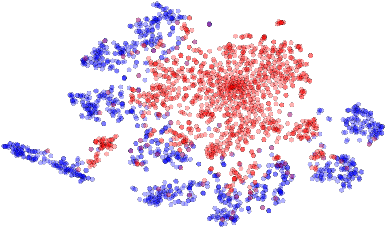
\includegraphics[width=0.45\textwidth]{./figures/adaptation_vis/pool2_mnist2inv_before.pdf}}\hfill%
  \subfigure[Adapted]{%%
    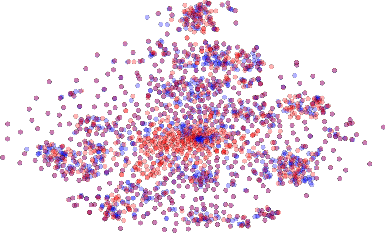
\includegraphics[width=0.45\textwidth]{./figures/adaptation_vis/pool2_mnist2inv_after.pdf}}%%
  \hspace*{\fill}%
  \end{minipage}%
  \begin{minipage}{.5\textwidth}
  \centering
  \small{{\sc Syn Numbers $ \rightarrow $ SVHN}: last hidden layer of the label predictor}
  \setcounter{subfigure}{0}
  \hspace*{\fill}%
  \subfigure[Non-adapted]{%%
    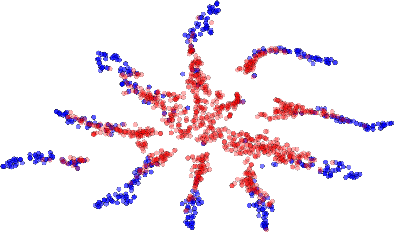
\includegraphics[width=0.45\textwidth]{./figures/adaptation_vis/before.pdf}}\hfill%
  \subfigure[Adapted]{%%
    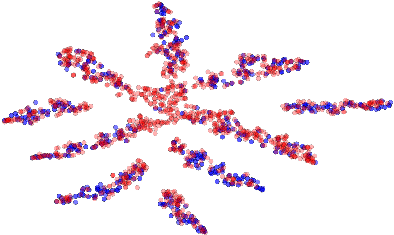
\includegraphics[width=0.45\textwidth]{./figures/adaptation_vis/after.pdf}}%%
  \hspace*{\fill}%
  \end{minipage}
  \caption{The effect of adaptation on the distribution of the extracted features (best viewed in color). The figure shows t-SNE \cite{Maaten13} visualizations of the CNN's activations {\bf (a)} in case when no adaptation was performed and {\bf (b)} in case when our adaptation procedure was incorporated into training. {\it Blue} points correspond to the source domain examples, while {\it red} ones correspond to the target domain. In all cases, the adaptation in our method makes the two distributions of features much closer.}
  \label{fig:exper_adapt_vis}
\end{figure*}

\subsection{Results}
\label{sect:exper_quant}

We now discuss the experimental settings and the results. In each case, we train on the source dataset and test on a different target domain dataset, with considerable shifts between domains (see \fig{exper_domains_examples}). The results are summarized in \tab{results} and \tab{results_office}. 

\vspace{2mm}\noindent {\bf MNIST $ \rightarrow $ MNIST-M.}
Our first experiment deals with the MNIST dataset~\cite{LeCun98} (source). In order to obtain the target domain ({\sc MNIST-M}) we blend digits from the original set over patches randomly extracted from color photos from BSDS500 \cite{Arbelaez11}. This operation is formally defined for two images $ I^{1}, I^{2} $ as $ I_{ijk}^{out} = | I_{ijk}^{1} - I_{ijk}^{2} | $, where $ i, j $ are the coordinates of a pixel and $ k $ is a channel index. In other words, an output sample is produced by taking a patch from a photo and inverting its pixels at positions corresponding to the pixels of a digit. For a human the classification task becomes only slightly harder compared to the original dataset (the digits are still clearly distinguishable) whereas for a CNN trained on MNIST this domain is quite distinct, as the background and the strokes are no longer constant. Consequently, the source-only model performs poorly. Our approach succeeded at aligning feature distributions (\fig{exper_adapt_vis}), which led to successful adaptation results (considering that the adaptation is unsupervised). At the same time, the improvement over source-only model achieved by subspace alignment (SA) \cite{Fernando13} is quite modest, thus highlighting the difficulty of the adaptation task. 

\vspace{2mm}\noindent {\bf Synthetic numbers $ \rightarrow $ SVHN.}
To address a common scenario of training on synthetic data and testing on  real data, we use Street-View House Number dataset {\sc SVHN} \cite{Netzer11} as the target domain and synthetic digits as the source. The latter ({\sc Syn ~Numbers}) consists of ~500,000 images generated by ourselves from Windows fonts by varying the text (that includes different one-, two-, and three-digit numbers), positioning, orientation, background and stroke colors, and the amount of blur. The degrees of variation were chosen manually to simulate SVHN, however the two datasets are still rather distinct, the biggest difference being the structured clutter in the background of SVHN images. 

The proposed backpropagation-based technique works well covering two thirds of the gap between training with source data only and training on target domain data with known target labels. In contrast, SA~\cite{Fernando13} does not result in any significant improvement in the classification accuracy, thus highlighting that the adaptation task is even more challenging than in the case of the MNIST experiment.

\vspace{2mm}\noindent {\bf MNIST $ \leftrightarrow $ SVHN.}
In this experiment, we further increase the gap between distributions, and test on {\sc MNIST} and {\sc SVHN}, which are significantly different in appearance. Training on SVHN even without adaptation is challenging --- classification error stays high during the first 150 epochs. In order to avoid ending up in a poor local minimum we, therefore, do not use learning rate annealing here. Obviously, the two directions ({\sc MNIST} $ \rightarrow $ {\sc SVHN} and {\sc SVHN} $ \rightarrow $ {\sc MNIST}) are not equally difficult. As {\sc SVHN} is more diverse, a model trained on SVHN is expected to be more generic and to perform reasonably on the MNIST dataset. This, indeed, turns out to be the case and is supported by the appearance of the feature distributions. We observe a quite strong separation between the domains when we feed them into the CNN trained solely on { \sc MNIST}, whereas for the {\sc SVHN}-trained network the features are much more intermixed. This difference probably explains why our method succeeded in improving the performance by adaptation in the {\sc SVHN} $ \rightarrow $ {\sc MNIST} scenario (see \tab{results}) but not in the opposite direction (SA is not able to perform adaptation in this case either). Unsupervised adaptation from MNIST to SVHN gives a failure example for our approach (we are unaware of any unsupervised DA methods capable of performing such adaptation).

\vspace{2mm}\noindent {\bf Synthetic Signs $ \rightarrow $ GTSRB.}
Overall, this setting is similar to the {\sc Syn Numbers} $ \rightarrow $ {\sc SVHN} experiment, except the distribution of the features is more complex due to the significantly larger number of classes (43 instead of 10). For the source domain we obtained~100,000 synthetic images (which we call {\sc Syn~Signs}) simulating various photoshooting conditions. Once again, our method achieves a sensible increase in performance once again proving its suitability for the synthetic-to-real data adaptation.

\begin{figure}
  \centering
  \setlength\figureheight{2.7cm}
  \setlength\figurewidth{6.8cm}
  % This file was created by matlab2tikz v0.5.0 running on MATLAB 8.3.
%Copyright (c) 2008--2014, Nico Schlömer <nico.schloemer@gmail.com>
%All rights reserved.
%Minimal pgfplots version: 1.3
%
%The latest updates can be retrieved from
%  http://www.mathworks.com/matlabcentral/fileexchange/22022-matlab2tikz
%where you can also make suggestions and rate matlab2tikz.
%
\begin{tikzpicture}[font=\scriptsize]

\begin{axis}[%
width=0.95092\figurewidth,
height=\figureheight,
at={(0\figurewidth,0\figureheight)},
scale only axis,
xmin=10000,
xmax=50000,
xlabel={Batches seen},
ymin=0,
ymax=1,
ylabel={Validation error},
axis x line*=bottom,
axis y line*=left,
legend style={at={($ (1,1) + (-0.1cm,-0.1cm) $)},anchor=north east,align=left,legend cell align=left,draw=black},
xmajorgrids,
ymajorgrids,
grid style={dashed}
]
\addplot [color=blue,solid,line width=1.0pt]
  table[row sep=crcr]{%
10500	0.199757996632997\\
11000	0.19162984006734\\
11500	0.190788089225589\\
12000	0.192918771043771\\
12500	0.196390993265993\\
13000	0.185527146464646\\
13500	0.190472432659933\\
14000	0.185606060606061\\
14500	0.183422769360269\\
15000	0.189051978114478\\
15500	0.191524621212121\\
16000	0.186079545454545\\
16500	0.179424452861953\\
17000	0.187684132996633\\
17500	0.187868265993266\\
18000	0.180923821548822\\
18500	0.187315867003367\\
19000	0.178661616161616\\
19500	0.18102904040404\\
20000	0.180555555555556\\
20500	0.176662457912458\\
21000	0.183791035353535\\
21500	0.179214015151515\\
22000	0.178898358585859\\
22500	0.178898358585859\\
23000	0.174479166666667\\
23500	0.174742213804714\\
24000	0.171059553872054\\
24500	0.177951388888889\\
25000	0.174794823232323\\
25500	0.174084595959596\\
26000	0.174636994949495\\
26500	0.169034090909091\\
27000	0.171191077441077\\
27500	0.170875420875421\\
28000	0.171506734006734\\
28500	0.170217803030303\\
29000	0.169244528619529\\
29500	0.169875841750842\\
30000	0.168744739057239\\
30500	0.17048085016835\\
31000	0.169454966329966\\
31500	0.167771464646465\\
32000	0.168849957912458\\
32500	0.168323863636364\\
33000	0.168718434343434\\
33500	0.165667087542088\\
34000	0.167376893939394\\
34500	0.169007786195286\\
35000	0.167140151515152\\
35500	0.165667087542088\\
36000	0.167850378787879\\
36500	0.169823232323232\\
37000	0.170691287878788\\
37500	0.16640361952862\\
38000	0.167981902356902\\
38500	0.169875841750842\\
39000	0.166771885521886\\
39500	0.169376052188552\\
40000	0.168087121212121\\
40500	0.165509259259259\\
41000	0.167718855218855\\
41500	0.168060816498317\\
42000	0.166035353535354\\
42500	0.166692971380471\\
43000	0.166429924242424\\
43500	0.167034932659933\\
44000	0.170349326599327\\
44500	0.169744318181818\\
45000	0.168218644781145\\
45500	0.166429924242424\\
46000	0.166324705387205\\
46500	0.168771043771044\\
47000	0.168034511784512\\
47500	0.168718434343434\\
48000	0.171059553872054\\
48500	0.170638678451178\\
49000	0.16819234006734\\
49500	0.168981481481481\\
50000	0.167902988215488\\
};
\addlegendentry{Real data only};

\addplot [color=cyan,solid,line width=1.0pt]
  table[row sep=crcr]{%
10500	0.9625\\
11000	0.79765625\\
11500	0.715625\\
12000	0.6140625\\
12500	0.52109375\\
13000	0.459375\\
13500	0.4484375\\
14000	0.421875\\
14500	0.39453125\\
15000	0.4109375\\
15500	0.34296875\\
16000	0.36875\\
16500	0.3359375\\
17000	0.36171875\\
17500	0.3171875\\
18000	0.3484375\\
18500	0.32421875\\
19000	0.315625\\
19500	0.346875\\
20000	0.31875\\
20500	0.35390625\\
21000	0.3265625\\
21500	0.33359375\\
22000	0.3171875\\
22500	0.28515625\\
23000	0.30546875\\
23500	0.309375\\
24000	0.2796875\\
24500	0.30859375\\
25000	0.30703125\\
25500	0.3078125\\
26000	0.28671875\\
26500	0.2875\\
27000	0.31484375\\
27500	0.2859375\\
28000	0.29375\\
28500	0.31328125\\
29000	0.3078125\\
29500	0.2859375\\
30000	0.2890625\\
30500	0.284375\\
31000	0.2953125\\
31500	0.26953125\\
32000	0.29921875\\
32500	0.30078125\\
33000	0.2640625\\
33500	0.309375\\
34000	0.2734375\\
34500	0.290625\\
35000	0.26796875\\
35500	0.3015625\\
36000	0.26796875\\
36500	0.2921875\\
37000	0.265625\\
37500	0.2765625\\
38000	0.2859375\\
38500	0.32109375\\
39000	0.28046875\\
39500	0.275\\
40000	0.24921875\\
40500	0.29140625\\
41000	0.26640625\\
41500	0.265625\\
42000	0.259375\\
42500	0.2765625\\
43000	0.26796875\\
43500	0.2765625\\
44000	0.27265625\\
44500	0.25546875\\
45000	0.26484375\\
45500	0.271875\\
46000	0.2703125\\
46500	0.26171875\\
47000	0.246875\\
47500	0.25078125\\
48000	0.29609375\\
48500	0.2640625\\
49000	0.26875\\
49500	0.26015625\\
50000	0.2578125\\
};
\addlegendentry{Synthetic data only};

\addplot [color=red,solid,line width=1.0pt]
  table[row sep=crcr]{%
10500	0.943892045454545\\
11000	0.943892045454545\\
11500	0.943892045454545\\
12000	0.943892045454545\\
12500	0.848300715488216\\
13000	0.658722643097643\\
13500	0.590593434343434\\
14000	0.475484006734007\\
14500	0.313946759259259\\
15000	0.235690235690236\\
15500	0.17879313973064\\
16000	0.152383207070707\\
16500	0.12912984006734\\
17000	0.114478114478114\\
17500	0.116214225589226\\
18000	0.1015625\\
18500	0.10066813973064\\
19000	0.101983375420875\\
19500	0.0914351851851852\\
20000	0.0895675505050505\\
20500	0.0894360269360269\\
21000	0.0827283249158249\\
21500	0.0798611111111111\\
22000	0.0859638047138047\\
22500	0.0799137205387205\\
23000	0.0778619528619529\\
23500	0.0737584175084175\\
24000	0.0742582070707071\\
24500	0.0776778198653199\\
25000	0.0771517255892256\\
25500	0.0725747053872054\\
26000	0.0739425505050505\\
26500	0.0734953703703704\\
27000	0.0730744949494949\\
27500	0.0688920454545455\\
28000	0.0702072811447811\\
28500	0.072337962962963\\
29000	0.0670244107744108\\
29500	0.0733638468013468\\
30000	0.0667613636363636\\
30500	0.0692340067340067\\
31000	0.0652093855218855\\
31500	0.0664720117845118\\
32000	0.0655776515151515\\
32500	0.0671296296296296\\
33000	0.0656039562289562\\
33500	0.0646043771043771\\
34000	0.0668665824915825\\
34500	0.0638678451178451\\
35000	0.065077861952862\\
35500	0.0649989478114478\\
36000	0.0672348484848485\\
36500	0.0668665824915825\\
37000	0.0626052188552189\\
37500	0.0652093855218855\\
38000	0.0626315235690236\\
38500	0.0627893518518518\\
39000	0.0613162878787879\\
39500	0.063236531986532\\
40000	0.0629208754208754\\
40500	0.0639467592592593\\
41000	0.0612899831649832\\
41500	0.0653409090909091\\
42000	0.0608691077441077\\
42500	0.0613425925925926\\
43000	0.0630260942760943\\
43500	0.060106271043771\\
44000	0.0638678451178451\\
44500	0.0602377946127946\\
45000	0.0577388468013468\\
45500	0.062684132996633\\
46000	0.0608164983164983\\
46500	0.0603167087542088\\
47000	0.0577651515151515\\
47500	0.0583175505050505\\
48000	0.0591329966329966\\
48500	0.0607112794612795\\
49000	0.0585805976430976\\
49500	0.0583175505050505\\
50000	0.0590540824915825\\
};
\addlegendentry{Both};

\end{axis}
\end{tikzpicture}%
  \caption{Semi-supervised domain adaptation for the traffic signs. As labeled target domain data are shown to the method, it achieves significantly lower error than the model trained on target domain data only or on source domain data only. \vspace{-4mm}}
  \label{fig:exper_semi_test}
\end{figure}

As an additional experiment, we also evaluate the proposed algorithm for semi-supervised domain adaptation, i.e.\ when one is additionally provided with a small amount of labeled target data. For that purpose we split {\sc GTSRB} into the train set (1280 random samples with labels) and the validation set (the rest of the dataset). The validation part is used solely for the evaluation and does not participate in the adaptation. The training procedure changes slightly as the label predictor is now exposed to the target data. \fig{exper_semi_test} shows the change of the validation error throughout the training. While the graph clearly suggests that our method can be used in the semi-supervised setting, thorough verification of semi-supervised setting is left for future work.


\vspace{2mm}\noindent {\bf Office dataset.} 
We finally evaluate our method on {\sc Office} dataset, which is a collection of three distinct domains: {\sc Amazon}, {\sc DSLR}, and {\sc Webcam}. Unlike previously discussed datasets, {\sc Office} is rather small-scale with only 2817 labeled images spread across 31 different categories in the largest domain. The amount of available data is crucial for a successful training of a deep model, hence we opted for the fine-tuning of the CNN pre-trained on the ImageNet \cite{Jia14} as it is done in some recent DA works \cite{Donahue14,Tzeng14,Hoffman14}. We make our approach more comparable with \cite{Tzeng14} by using exactly the same network architecture replacing domain mean-based regularization with the domain classifier.

Following most previous works, we evaluate our method using 5 random splits for each of the 3 transfer tasks commonly used for evaluation. Our training protocol is close to \cite{Tzeng14,Saenko10,Gong12} as we use the same number of labeled source-domain images per category. Unlike those works and similarly to e.g.\ DLID~\cite{Chopra13} we use the whole unlabeled target domain (as the premise of our method is the abundance of unlabeled data in the target domain). Under this transductive setting, our method is able to improve previously-reported state-of-the-art accuracy for unsupervised adaptation very considerably (\tab{results_office}), especially in the most challenging {\sc Amazon} $ \rightarrow $ {\sc Webcam} scenario (the two domains with the largest domain shift).


\section{VQA Dataset Analysis}
\label{sec:analysis}
%\vspace{\sectionReduceBot}
%%%%%%%%%%%%%%%%%%%%%%%%%%%%%%%%%%%%%%%%%%%%%%%%%%%%%%%%%%%
%%%%%%%%%%%%%%%%%%%%%%%%%%%%%%%%%%%%%%%%%%%%%%%%%%%%%%%%%%%
\begin{figure*}[t]
\centering
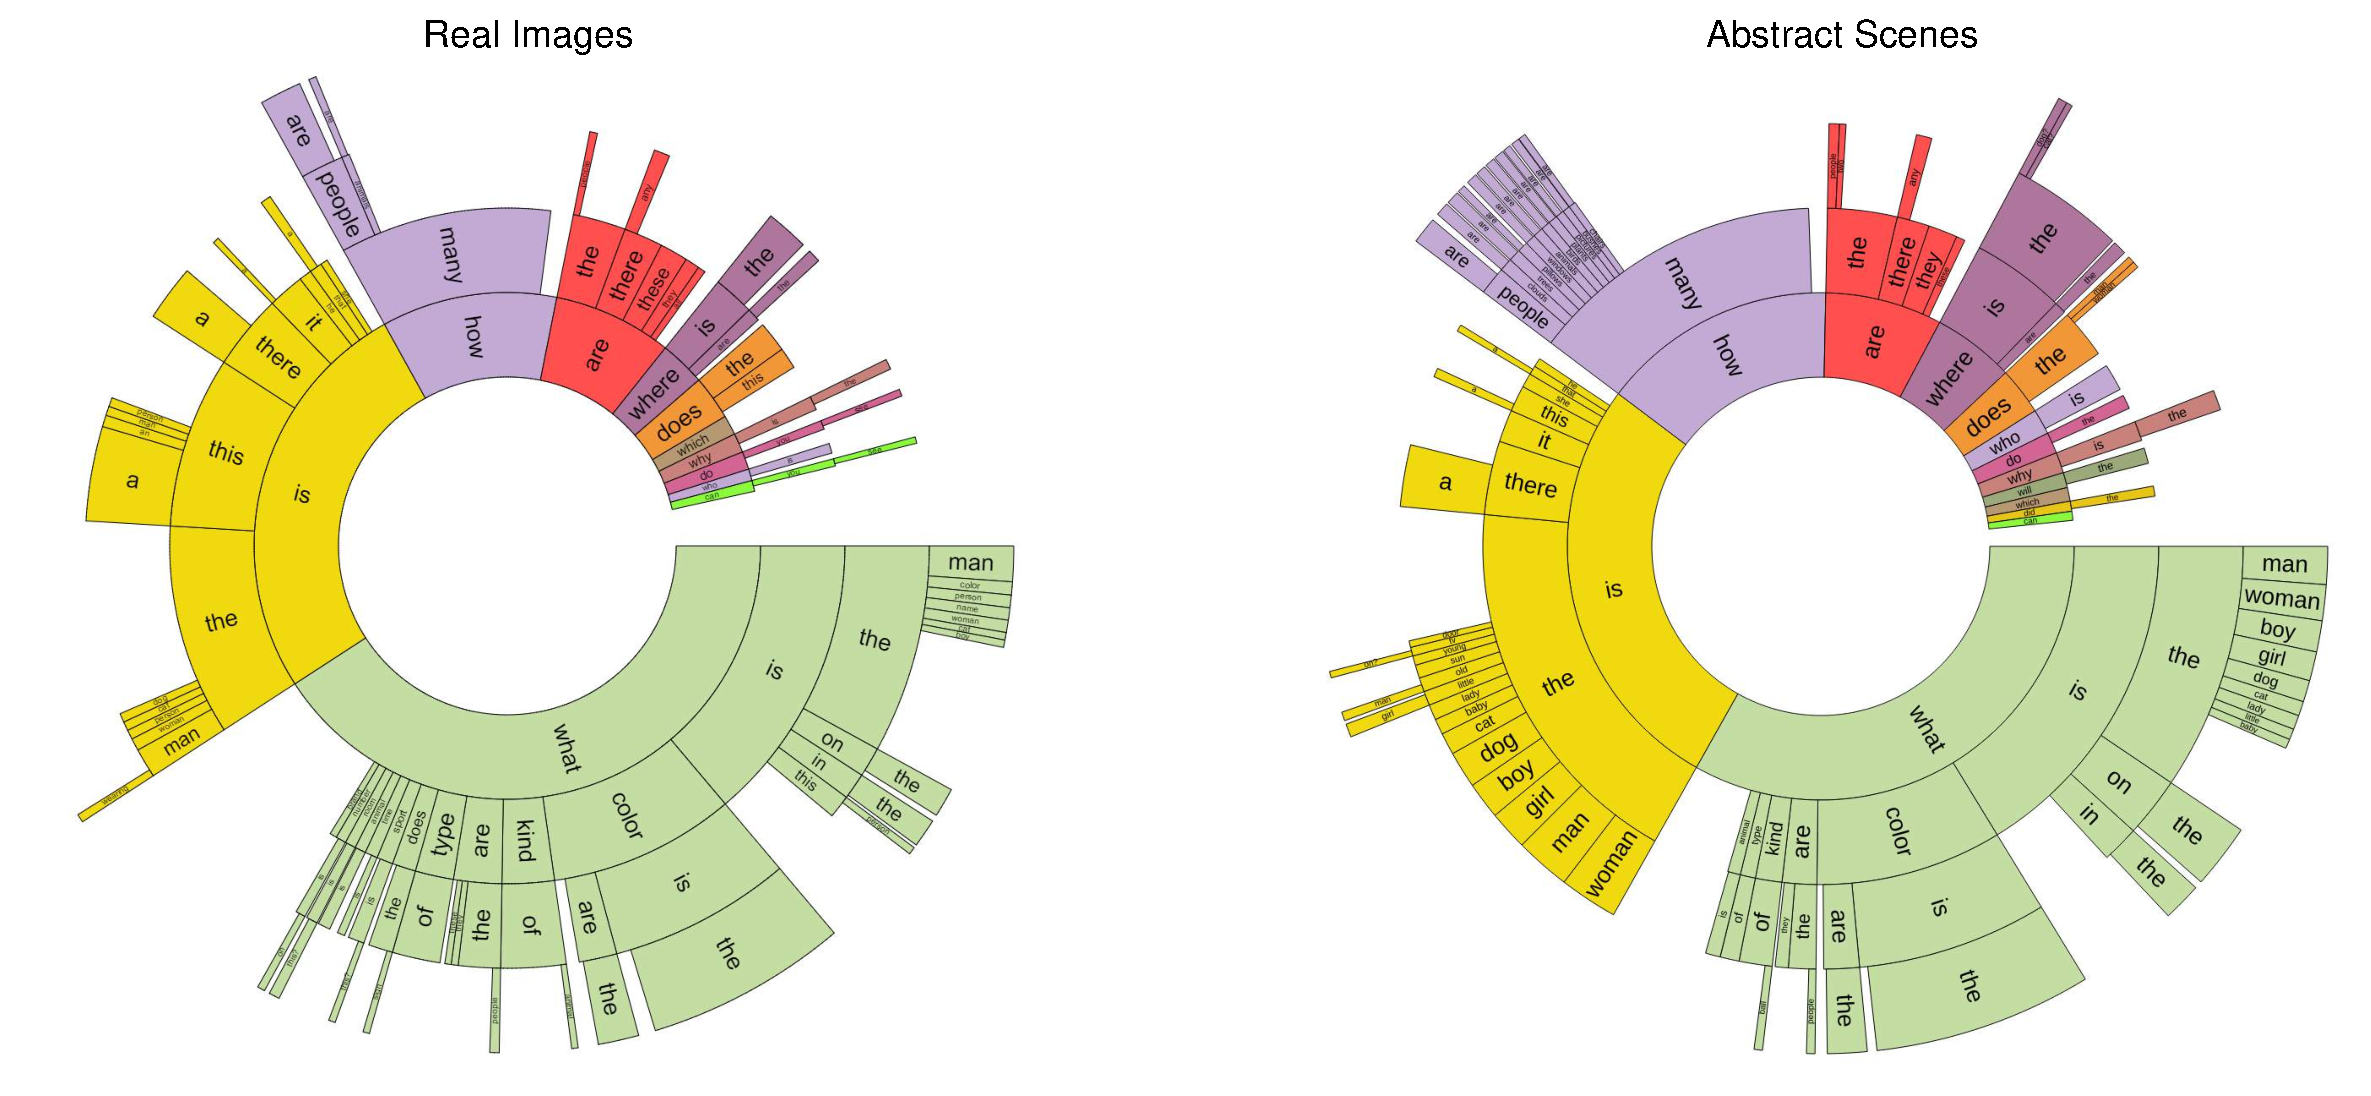
\includegraphics[width=1\linewidth]{figures/QuestionTypes3.pdf}
\caption{Distribution of questions by their first four words for a random sample of 60K questions for real images (left) and all questions for abstract scenes (right). The ordering of the words starts towards the center and radiates outwards. The arc length is proportional to the number of questions containing the word. White areas are words with contributions too small to show. }
%\vspace{-5pt}
\label{fig:QuesCluster}
%\setlength{\belowcaptionskip}{-10pt}
\end{figure*}
%%%%%%%%%%%%%%%%%%%%%%%%%%%%%%%%%%%%%%%%%%%%%%%%%%%%%%%%%%%

In this section, we provide an analysis of the questions and answers in the VQA train dataset.
To gain an understanding of the types of questions asked and answers provided, we visualize
the distribution of question types and answers. We also explore how often the questions may
be answered without the image using just commonsense information. Finally, we analyze whether
the information contained in an image caption is sufficient to answer the questions.

The dataset includes 614,163 questions 
%and a total of 
and 7,984,119 answers (including answers provided by workers with and without 
looking at the image) 
%and without looking at the image) 
for 204,721 images from the MS COCO dataset~\cite{coco} and 150,000 questions with 1,950,000 answers for $50,000$ abstract scenes.

%\textcolor{red}{
%We emphasize that the creation of a dataset of this scale and richness
%is a time consuming process, taking months to complete.
%While the entirety of the dataset has been collected,} at the time of original submission,
%120,520 questions with 270,210 answers for 50,000 MS COCO
%images and 30,000 questions with 79,740 answers for 10,000 abstract scenes had been collected.
%Please refer to the appendix for further details.
%\textcolor{red}{The results in this section still reflect that subset of the final dataset.}
%We emphasize that the creation of a dataset of this scale and richness
%is a time consuming process, taking months to complete.
%By our current estimates,
%approximately 5,000 questions and 40,000 answers are collected per day
%using Amazon Mechanical Turk (AMT).
%The entire dataset will take approximately three months to complete. At the time of submission,
%120,520 questions with 270,210 answers for 50,000 MS COCO
%images and 30,000 questions with 79,740 answers for 10,000 abstract scenes had been collected.
%Please refer to the appendix for further details.


%%%%%%%%%%%%%%%%%%%%%%%%%%%%%%%%%%%%%%%%%%%%%%%%%%%%%%%%%%%
%\vspace{\subsectionReduceTop}
\subsection{Questions}
%\vspace{\subsectionReduceBot}
%%%%%%%%%%%%%%%%%%%%%%%%%%%%%%%%%%%%%%%%%%%%%%%%%%%%%%%%%%%

\textbf{Types of Question.}
Given the structure of questions generated in the English language,
we can cluster questions into different types based on the words that start the question.
\figref{fig:QuesCluster} shows the distribution of questions based on the first four
words of the questions for both the real images (left) and abstract scenes (right).
Interestingly, the distribution of questions is quite similar for both real images and abstract scenes.
This helps demonstrate that the type of questions elicited by the abstract scenes is similar to
those elicited by the real images. There exists a surprising variety of question types,
including ``What is$\ldots$'', ``Is there$\ldots$'', ``How many$\ldots$'', and ``Does the$\ldots$''.
Quantitatively, the percentage of questions for different types is shown in \tableref{tab:typeacc}. Several example questions and answers are shown in \figref{fig:qualResults}.
%\textbf{Sub-Types.}
A particularly interesting type of question is the ``What is$\ldots$'' questions, since they have a
diverse set of possible answers. See the appendix for visualizations for ``What is$\ldots$'' questions.

\textbf{Lengths.}
\figref{fig:QuesLen} shows the distribution of question lengths.
We see that most questions range from four to ten words.


\begin{comment}\begin{table}[h]
{\small
\begin{tabular}{@{\extracolsep{\fill}}p{2cm}|ccccc@{\extracolsep{\fill}}}
%\toprule
Dataset  & Yes & No\\
%\midrule
Real   & 18.21 & 14.06 \\
Abstract & 26.54 & 16.70 \\
\end{tabular}
}
\vspace{5pt}
\caption{Percentage of ``yes'' and ``no'' questions in the real and abstract datasets.}
\label{table:yesno}
%\vspace{\captionReduceBot}
\end{table}
\end{comment}

%%%%%%%%%%%%%%%%%%%%%%%%%%%%%%%%%%%%%%%%%%%%%%%%%%%%%%%%%%%
\begin{figure}[t]
\centering
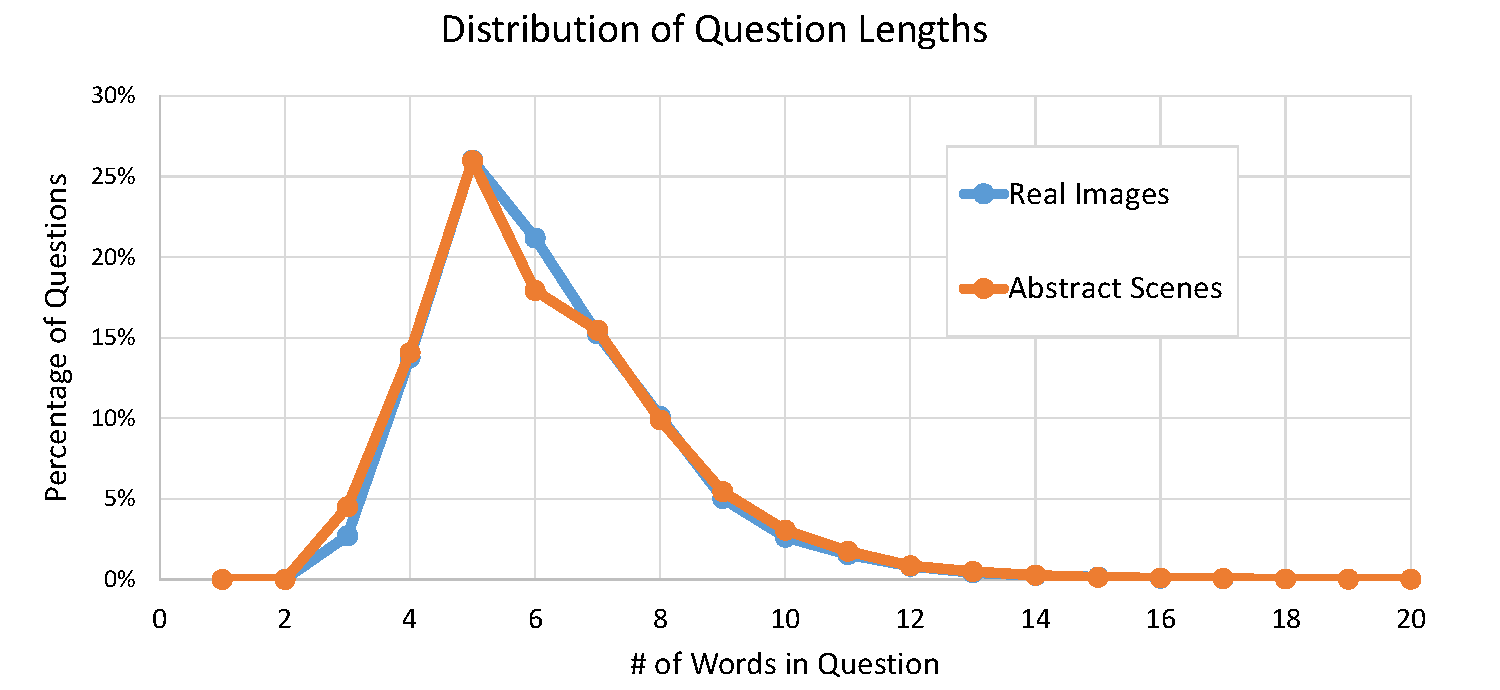
\includegraphics[width=1\linewidth]{figures/Lengths.pdf}
%\vspace{-9pt}
\caption{Percentage of questions with different word lengths for real images and abstract scenes.}
%\vspace{-5pt}
\label{fig:QuesLen}
%\setlength{\belowcaptionskip}{-10pt}
\end{figure}
%%%%%%%%%%%%%%%%%%%%%%%%%%%%%%%%%%%%%%%%%%%%%%%%%%%%%%%%%%%




\begin{figure*}
\centering
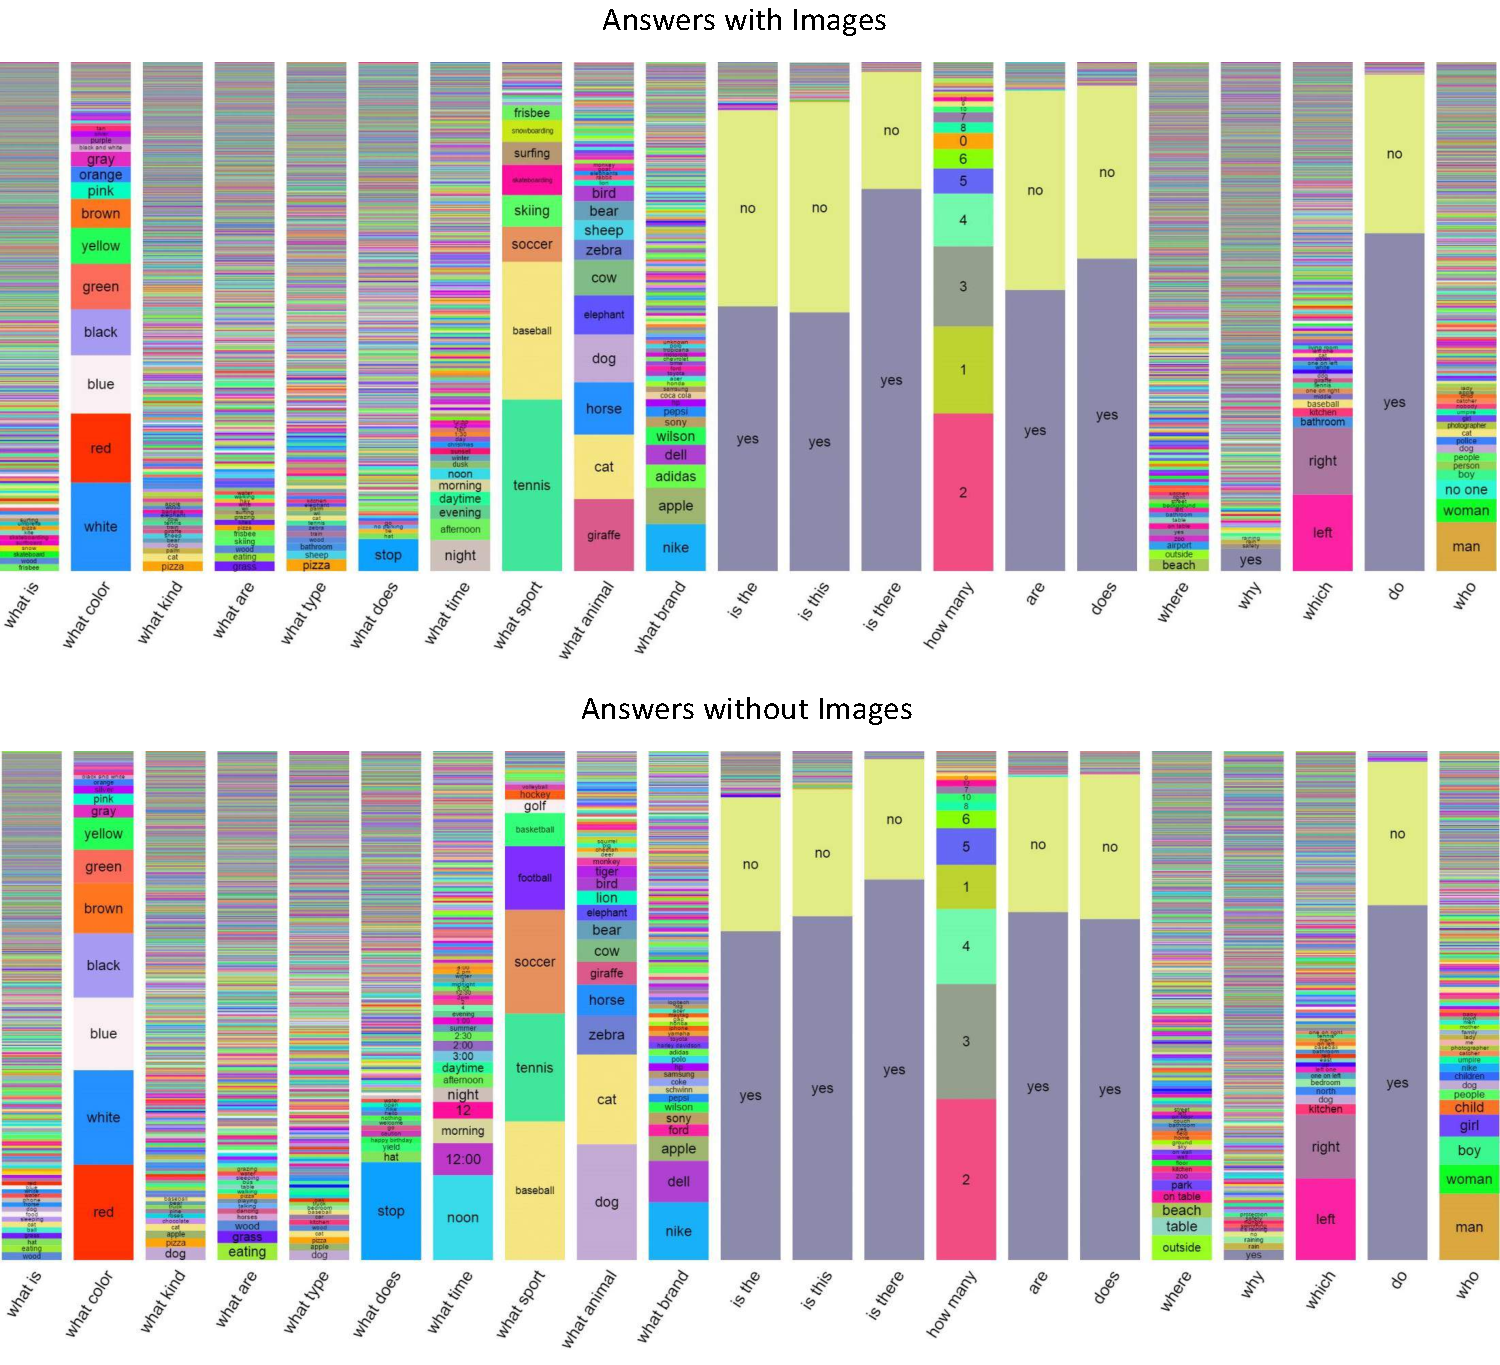
\includegraphics[width=1\linewidth]{figures/answers.pdf}
%\vspace{-5pt}
\caption{Distribution of answers per question type for a random sample of 60K questions for real images when subjects provide answers when given the image (top) and when not given the image (bottom).}
%\vspace{-5pt}
\label{fig:AnsPerQues}
%\setlength{\belowcaptionskip}{-10pt}
\end{figure*}


%%%%%%%%%%%%%%%%%%%%%%%%%%%%%%%%%%%%%%%%%%%%%%%%%%%%%%%%%%%
%\vspace{\subsectionReduceTop}
\subsection{Answers}
%\vspace{\subsectionReduceBot}
%%%%%%%%%%%%%%%%%%%%%%%%%%%%%%%%%%%%%%%%%%%%%%%%%%%%%%%%%%%

%\textbf{Typical Answers for Different Question Types.}
\textbf{Typical Answers.}
%Next, we analyze the answers provided for different question types.
\figref{fig:AnsPerQues} (top) shows the distribution of answers for several question types.
We can see that a number of question types, such as ``Is the\ldots'', ``Are\ldots'', and ``Does\ldots'' are
typically answered using ``yes'' and ``no'' as answers.
%\textcolor{red}{Question types such as ``How many\ldots'' are answered using numbers. $12.31\%$ and $14.48\%$ of the questions are answered using numbers on real images and abstract scenes, respectively.}
Other questions such as ``What is\ldots'' and ``What type\ldots'' have a rich diversity
of responses. Other question types such as ``What color\ldots'' or ``Which\ldots'' have more specialized responses,
such as colors, or ``left'' and ``right''. 
See the appendix for a list of the most popular answers.

\textbf{Lengths.}
Most answers consist of a single word, with the distribution of answers containing one, two, or three words, respectively being $89.32\%$, $6.91\%$, and $2.74\%$ for real images and $90.51\%$, $5.89\%$, and $2.49\%$ for abstract scenes.
%$89.16\%$, $7.00\%$, and $2.77\%$ of answers containing one, two, or three words, respectively.
The brevity of answers is not surprising, since the questions tend to elicit specific
information from the images. This is in contrast with image captions that generically
describe the entire image and hence tend to be longer. The brevity of our answers makes
automatic evaluation feasible. While it may be tempting to believe the brevity of the answers
makes the problem easier, recall that they are human-provided open-ended answers to
open-ended questions. The questions typically require complex reasoning to arrive at these
deceptively simple answers (see \figref{fig:qualResults}).
There are currently 23,234 unique one-word answers in our dataset for real images and 3,770 for abstract scenes.
%There are currently 10,011 unique one-word answers in our dataset.

\textbf{`Yes/No' and `Number' Answers.}
Many questions are answered using either ``yes'' or ``no'' (or sometimes ``maybe'') -- 
$38.37\%$ and $40.66\%$ of the questions on real images and abstract scenes respectively. 
Among these `yes/no' questions, there is a bias towards %answering with 
``yes'' -- %with ``yes'' being preferred %$61.32\%$ and $58.46\%$ 
$58.83\%$ and $55.86\%$ of `yes/no' answers are ``yes'' for real images and abstract scenes. 
Question types such as ``How many\ldots'' are answered using numbers -- 
$12.31\%$ and $14.48\%$ of the questions on real images and abstract scenes are `number' questions. 
``2'' is the most popular answer among the `number' questions, making up 
$26.04\%$ of the `number' answers for real images and $39.85\%$ for abstract scenes. 

\textbf{Subject Confidence.}
When the subjects answered the questions, we asked
``Do you think you were able to answer the question correctly?''.
\figref{fig:ConfScores} shows the distribution of responses. A majority of the answers
were labeled as confident for both real images and abstract scenes. % respectively.

\textbf{Inter-human Agreement.}
Does the self-judgment of confidence correspond to the answer agreement between subjects?
\figref{fig:ConfScores} shows the percentage of questions in which 
(i) $7$ or more, 
(ii) $3-7$, or 
(iii) less than $3$ subjects agree on the answers given their average confidence score 
(0 = not confident, 1 = confident).
As expected, the agreement between subjects increases with confidence.
However, even if all of the subjects are confident the answers may still vary.
This is not surprising since some answers may vary, yet have very similar meaning, such as ``happy'' and ``joyful''.

\begin{figure}[t]
\centering
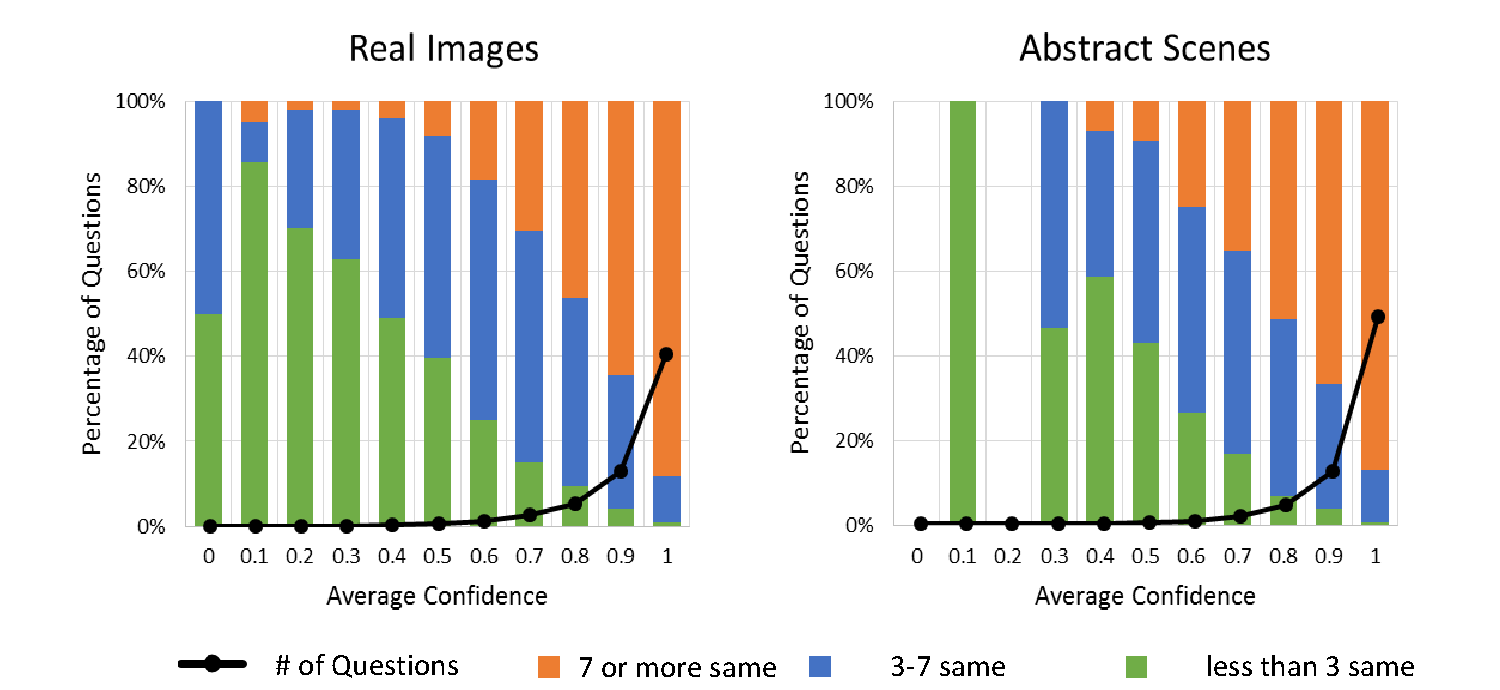
\includegraphics[width=1\linewidth]{figures/Confidence.pdf}
%\vspace{-5pt}
\caption{Number of questions per average confidence score (0 = not confident, 1 = confident) for real images and abstract scenes (black lines). Percentage of questions where 7 or more answers are same, 3-7 are same, less than 3 are same (color bars). }
%\vspace{-7pt}
\label{fig:ConfScores}
%\setlength{\belowcaptionskip}{-10pt}
\end{figure}

As shown in \tableref{table:commonsense_acc} (Question + Image), there is significant inter-human
agreement in the answers for both real images ($83.30\%$) and abstract scenes ($87.49\%$). 
%when humans are provided both the question and image while answering the question.
Note that on average each question has $2.70$ unique answers for real images and $2.39$ for abstract scenes. 
The agreement is significantly higher ($>95\%$) for \quotes{yes/no} questions and lower for other questions ($<76\%$), possibly due to the fact that we perform exact string matching and do not account for synonyms, plurality, \etc. Note that the automatic determination of synonyms is a difficult problem, since the level of answer granularity can vary across questions.




%%%%%%%%%%%%%%%%%%%%%%%%%%%%%%%%%%%%%%%%%%%%%%%%%%%%%%%%%%%
%\vspace{\subsectionReduceTop}
\subsection{Commonsense Knowledge}
\label{sec:cs}
%\vspace{\subsectionReduceBot}
%%%%%%%%%%%%%%%%%%%%%%%%%%%%%%%%%%%%%%%%%%%%%%%%%%%%%%%%%%%
\begin{figure*}[t]
 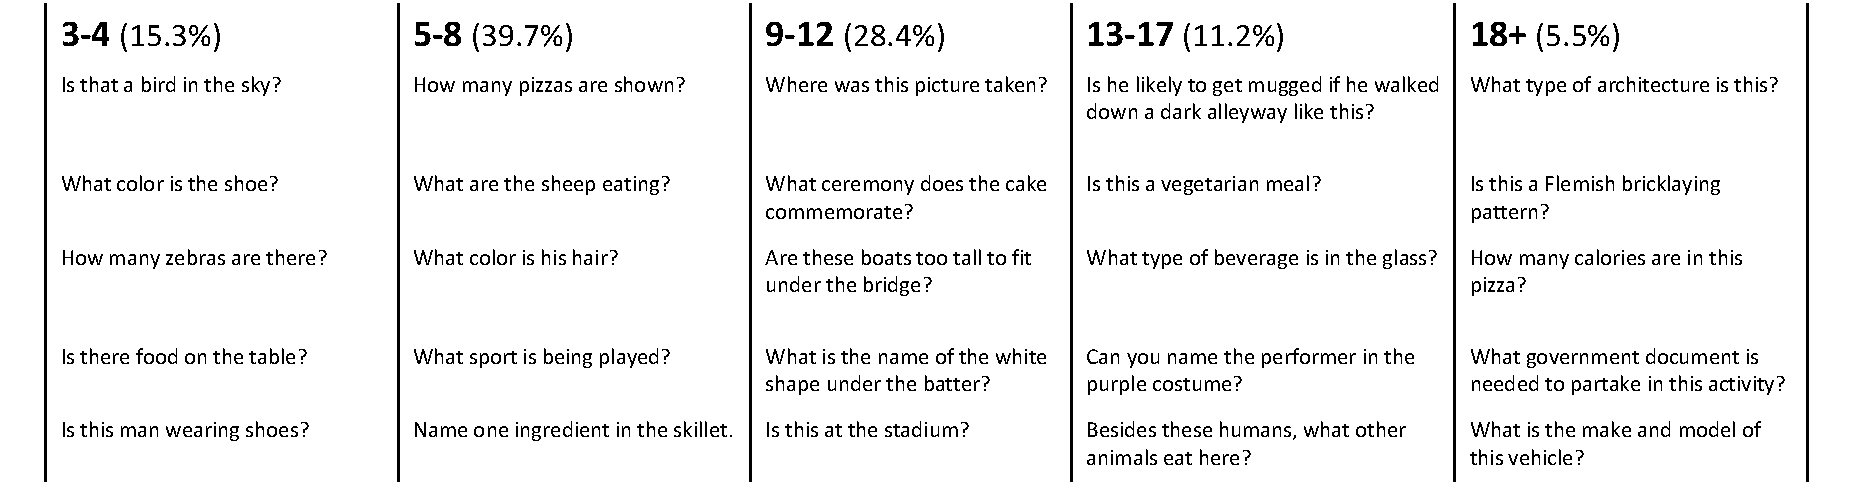
\includegraphics[width=\linewidth]{figures/age.pdf}
 \centering
\caption{\small Example questions judged by Mturk workers to be answerable by different age groups. The percentage of questions falling into each age group is shown in parentheses.}
 \label{fig:age}
 \end{figure*}
 	
\textbf{Is the Image Necessary?}
%Can the questions be answered using commonsense knowledge alone without the need for an image,
%\eg, ``What is the color of the sheep?''?
Clearly, some questions can sometimes be
answered correctly using commonsense knowledge alone without the need for an image,
\eg, ``What is the color of the fire hydrant?''.
We explore this issue by asking three subjects to answer
the questions \emph{without seeing the image} (see the examples in blue in \figref{fig:qualResults}).
In \tableref{table:commonsense_acc} (Question), we show the percentage of questions for which
the correct answer is provided over all questions, ``yes/no'' questions, and the other questions that
are not ``yes/no''. For ``yes/no'' questions, the human subjects respond better than chance.
For other questions, humans are only correct about $21\%$ of the time. This demonstrates that
understanding the visual information is critical to VQA and that commonsense information alone is not sufficient.

To show the qualitative difference in answers provided with and without images,
we show the distribution of answers for various question types in \figref{fig:AnsPerQues} (bottom).
The distribution of colors, numbers, and even ``yes/no'' responses is surprisingly different for answers
with and without images.
 
\textbf{Which Questions Require Common Sense?}
In order to identify questions that require commonsense reasoning to answer, we conducted 
two AMT studies (on a subset 10K questions from the real images of VQA trainval) asking subjects --
\begin{compactenum} 
\item Whether or not they believed a question required commonsense to answer the question, and 
\item The youngest age group that they believe a person must be in order to be able to correctly answer the question -- 
toddler (3-4), 
younger child (5-8), 
older child (9-12), 
teenager (13-17), 
adult (18+).
\end{compactenum}
Each question was shown to 10 subjects. We found that 
for $47.43\%$ of questions 3 or more subjects voted `yes' to commonsense, 
($18.14\%$: 6 or more).  
In the `perceived human age required to answer question' study, we found the following distribution of responses: 
toddler: $15.3\%$,
younger child: $39.7\%$, 
older child: $28.4\%$, 
teenager: $11.2\%$, 
adult: $5.5\%$.
In Figure \ref{fig:age} we show several questions for which a majority of subjects picked the specified age range. Surprisingly the perceived age needed to answer the questions is fairly well distributed across the different age ranges. As expected the questions that were judged answerable by an adult (18+) generally need specialized knowledge, whereas those answerable by a toddler (3-4) are more generic.
 
We measure the degree of commonsense required to answer a question as the percentage of subjects (out of 10) who voted ``yes'' in our ``whether or not a question requires commonsense'' study.
A fine-grained breakdown of average age and average degree of common sense (on a scale of $0-100$) required to answer a question is shown in \tableref{tab:typeacc}. The average age and the average degree of commonsense across all questions is $8.92$ and $31.01\%$ respectively. 

%\arxiv{To compute average age and average degree of commonsense across questions, we first compute the average age and average degree of commonsense (binary response scaled to $0-100$) per question (by taking average across 10 subjects for each question) and then take average across questions.} 

It is important to distinguish between:
\begin{compactenum}
\item How old someone needs to be to be able to answer a question correctly,  and
\item How old people \emph{think} someone needs to be to be able to answer a question correctly. 
\end{compactenum}

Our age annotations capture the latter -- perceptions of MTurk workers in an uncontrolled environment. As such, the relative ordering of question types in \tableref{tab:typeacc} is more important than absolute age numbers.
%The relative ordering of question types is more important than the absolute age numbers. It is important to note that the age annotations we have collected are just perceived ages: how old people -- untrained MTurk workers in an uncontrolled environment -- \emph{think} someone needs to be to be able to answer a question correctly.}
The two rankings of questions in terms of common sense required according to the two studies 
were largely correlated (Pearson's rank correlation: 0.58). 

%%%%%%%%%%%%%%%%%%%%%%%%%%%%%%%%%%%%%%%%%%%%%%%%%%%%%%%%%%%
\begin{table}[t]
\setlength{\tabcolsep}{3.2pt}
{\small
\begin{center}
%\begin{tabular}{@{}llccc@{}}
%\toprule
%Dataset & Input & All & Yes/No & Other \\
%%\hline
%\midrule
%    & Question & 40.81 & 67.60 & 21.22 \\
%Real   & Question + Caption* & 57.47 & 78.97 & 44.41 \\
%    & Question + Image & 83.30 & 95.77 & 72.67 \\
%%\hline
%\midrule
% & Question & 43.27 & 66.65 &  23.66 \\
%Abstract & Question + Caption* & 54.34 & 74.70 & 40.18 \\
% & Question + Image & 87.49 & 95.96 & 75.33 \\
%\bottomrule
%\end{tabular}
\begin{tabular}{@{}llcccc@{}}
\toprule
Dataset & Input & All & Yes/No & Number & Other \\
%\hline
\midrule
    & Question & 40.81 & 67.60 & 25.77 & 21.22 \\
Real   & Question + Caption* & 57.47 & 78.97 & 39.68 & 44.41 \\
    & Question + Image & 83.30 & 95.77 & 83.39 & 72.67 \\
%\hline
\midrule
 & Question & 43.27 & 66.65 & 28.52 & 23.66 \\
Abstract & Question + Caption* & 54.34 & 74.70 & 41.19 & 40.18 \\
 & Question + Image & 87.49 & 95.96 & 95.04 & 75.33 \\
\bottomrule
\end{tabular}
\end{center}
}
%\vspace{-7pt}
\caption {Test-standard accuracy of human subjects when asked to answer the 
question without seeing the image (Question), 
seeing just a caption of the image and not the image itself (Question + Caption), 
and seeing the image (Question + Image). 
Results are shown for all questions, ``yes/no'' \& ``number'' questions, and other questions 
that are neither answered ``yes/no'' nor number. 
All answers are free-form and not multiple-choice. 
*\hspace{1pt}These accuracies are evaluated on a subset of 3K train questions (1K images).}
% \textcolor{red}{and are not directly comparable to the corresponding numbers in older version.}}
\label{table:commonsense_acc}
%\vspace{\captionReduceBot}
%\vspace{-5pt}
\end{table}
%%%%%%%%%%%%%%%%%%%%%%%%%%%%%%%%%%%%%%%%%%%%%%%%%%%%%%%%%%%


%%%%%%%%%%%%%%%%%%%%%%%%%%%%%%%%%%%%%%%%%%%%%%%%%%%%%%%%%%%
%\vspace{\subsectionReduceTop}
\subsection{Captions \textbf{\vs} Questions}
%\vspace{\subsectionReduceBot}
%%%%%%%%%%%%%%%%%%%%%%%%%%%%%%%%%%%%%%%%%%%%%%%%%%%%%%%%%%%


Do generic image captions provide enough information to answer the questions?
\tableref{table:commonsense_acc} (Question + Caption) shows the percentage of questions answered
correctly when human subjects are given the question and a human-provided caption
describing the image, but not the image. As expected, the results are better than when humans are shown the questions alone.
However, the accuracies are significantly lower than when subjects are shown the actual image.
This demonstrates that in order to answer the questions correctly, deeper image understanding 
(beyond what image captions typically capture) is necessary. In fact, we find that the distributions of nouns, verbs, and adjectives mentioned in captions is statistically significantly different from those mentioned in our questions + answers (Kolmogorov-Smirnov test, $p<.001$) for both real images and abstract scenes. See the appendix for details. 
%This motivates the VQA task as a way to learn further information about visual scenes.

\section{Related work}\label{s:related}

\begin{figure}[t]
\centering
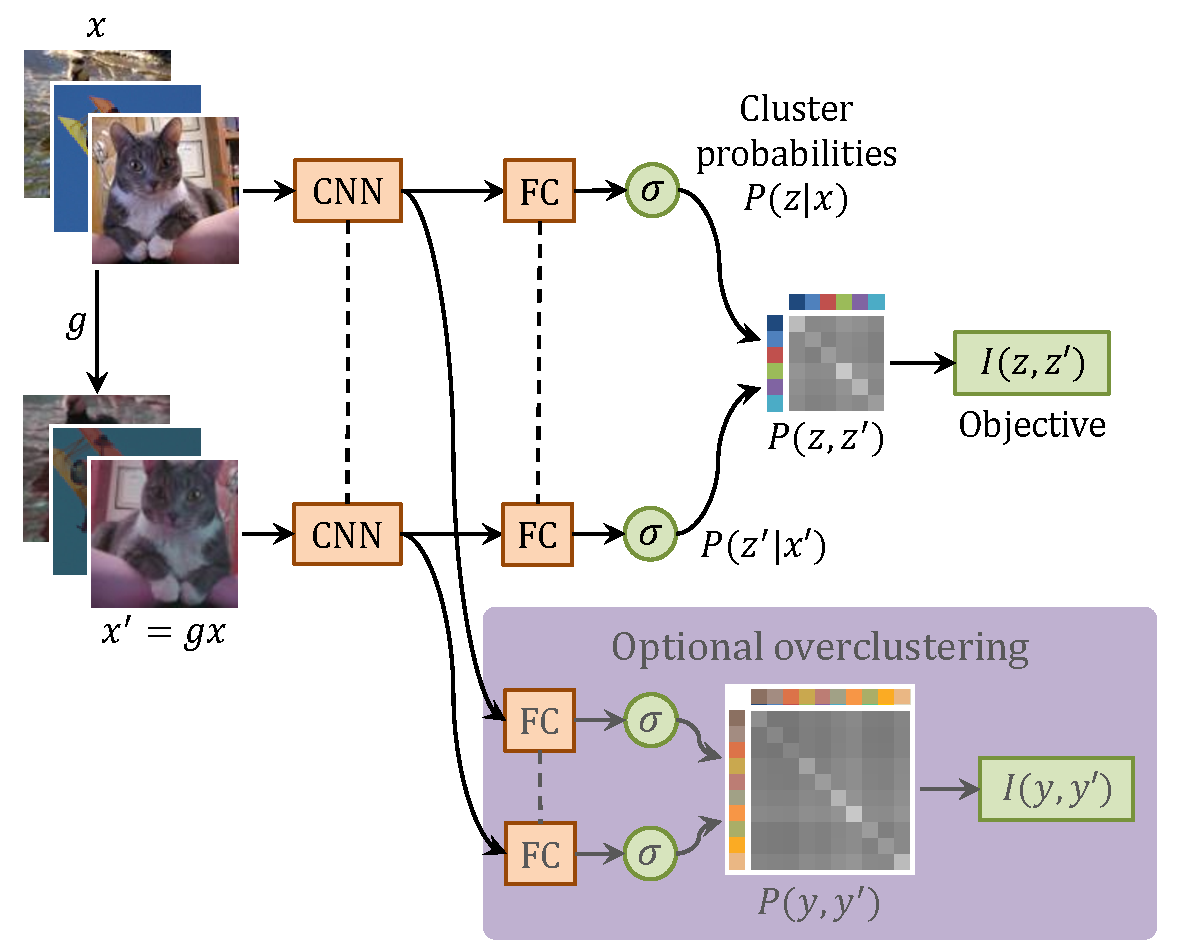
\includegraphics[width=0.95\columnwidth]{paper_imgs/overview1.pdf}
\caption{\label{f:overview}\methodnameshort for image clustering. Dashed line denotes shared parameters, $g$ is a random transformation, and $I$ denotes mutual information~(\cref{e:loss_expanded}).}
\end{figure}


\begin{figure*}
%\captionsetup{justification=centering}
\setlength\tabcolsep{2.2pt} % default value: 6pt

\begin{tabular}{c c c c c c}
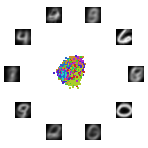
\includegraphics[height=0.16\textwidth]{experiments2_files/mnist_progression/726_run_1_colour_0_pointcloud_0.png} & 
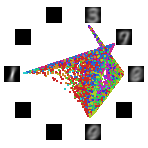
\includegraphics[height=0.16\textwidth]{experiments2_files/mnist_progression/726_run_1_colour_0_pointcloud_3.png} & 
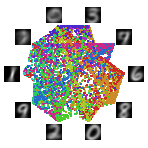
\includegraphics[height=0.16\textwidth]{experiments2_files/mnist_progression/726_run_1_colour_0_pointcloud_10.png} & 
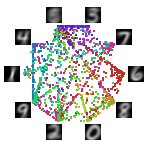
\includegraphics[height=0.16\textwidth]{experiments2_files/mnist_progression/726_run_1_colour_0_pointcloud_30.png} & 
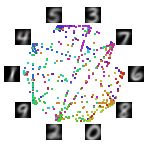
\includegraphics[height=0.16\textwidth]{experiments2_files/mnist_progression/726_run_1_colour_0_pointcloud_101.png} & 
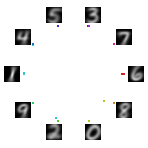
\includegraphics[height=0.16\textwidth]{experiments2_files/mnist_progression/726_run_1_colour_0_pointcloud_1000.png} 
\end{tabular}

\caption{\label{f:mnist_dots} Training with \methodnameshort on unlabelled MNIST in successive epochs from random initialisation (left). The network directly outputs cluster assignment probabilities for input images, and each is rendered as a coordinate by convex combination of 10 cluster vertices. There is no cherry-picking as the entire dataset is shown in every snapshot. Ground truth labelling (unseen by model) is given by colour. At each cluster the average image of its assignees is shown. With neither labels nor heuristics, the clusters discovered by \methodnameshort correspond perfectly to unique digits, with one-hot certain prediction (right).}
\end{figure*}


\paragraph{Co-clustering and mutual information.}

The use of information as a criterion to learn representations is not new. One of the earliest works to do so is by Becker and Hinton~\cite{becker1992self}.
More generally, learning from paired data has been explored in co-clustering~\cite{hartigan1972direct, dhillon2003information} and in other works~\cite{wang2010information} that build on the information bottleneck principle~\cite{friedman2001multivariate}.

Several recent papers have used information as a tool to train deep networks in particular.
IMSAT~\cite{hu2017learning} maximises mutual information between data and its representation and DeepINFOMAX~\cite{hjelm2018learning} maximizes information between spatially-preserved features and compact features.
However, IMSAT and DeepINFOMAX combine information with other criteria, whereas in our method information is the only criterion used.
Furthermore, both IMSAT and DeepINFOMAX compute mutual information over continuous random variables, which requires complex estimators~\cite{belghazi2018mine}, whereas \methodnameshort does so for discrete variables with simple and exact computations.
Finally, DeepINFOMAX considers the information $I(\bx, f(\bx))$ between the features $\bx$ and a deterministic function $f(\bx)$ of it, which is in principle the same as the entropy $H(\bx)$; in contrast, in \methodnameshort information does not trivially reduce to  entropy.

\paragraph{Semantic clustering versus intermediate representation learning.}
In semantic clustering, the learned function directly outputs discrete assignments for high level (i.e. semantic) clusters. Intermediate representation learners, on the other hand, produce continuous, distributed, high-dimensional representations that must be post-processed, for example by k-means, to obtain the discrete low-cardinality assignments required for unsupervised semantic clustering. The latter includes objectives such as generative autoencoder image reconstruction~\cite{vincent2010stacked},  triplets~\cite{schultz2004learning} and spatial-temporal order or context prediction~\cite{lee2017unsupervised,cruz2017deeppermnet,doersch2015unsupervised}, for example predicting patch proximity~\cite{isola2015learning}, solving jigsaw puzzles~\cite{noroozi2016unsupervised} and inpainting~\cite{pathak2016context}. Note it also includes a number of clustering methods (DeepCluster~\cite{caron2018deep}, exemplars~\cite{dosovitskiy2015discriminative}) where the clustering is only auxiliary; a clustering-style objective is used but does not produce groups with semantic correspondence. For example, DeepCluster~\cite{caron2018deep} is a state-of-the-art method for learning highly-transferable intermediate features using overclustering as a proxy task, but does not automatically find semantically meaningful clusters. As these methods use auxiliary objectives divorced from the semantic clustering objective, it is unsurprising that they perform worse than \methodnameshort~(\cref{s:experiments}), which directly optimises for it, training the network end-to-end with the final clusterer implicitly wrapped inside.




\paragraph{Optimising image-to-image distance.}

Many approaches to deep clustering, whether semantic or auxiliary, utilise a distance function between input images that approximates a given grouping criterion.
Agglomerative clustering~\cite{bautista2016cliquecnn} and partially ordered sets~\cite{bautista2017deep} of HOG features~\cite{dalal2005histograms} have been used to group images, and exemplars~\cite{dosovitskiy2015discriminative} define a group as a set of random transformations applied to a single image. Note the latter does not scale easily, in particular to image segmentation where a single $200\times 200$ image would call for 40k classes. DAC~\cite{chang2017deep}, JULE~\cite{yang2016joint}, DeepCluster~\cite{caron2018deep}, ADC~\cite{haeusser2018associative} and DEC~\cite{xie2016unsupervised} rely on the inherent visual consistency and disentangling properties~\cite{greff2015binding} of CNNs to produce cluster assignments, which are processed and reinforced in each iteration. 
The latter three are based on k-means style mechanisms to refine feature centroids, which is prone to degenerate solutions~\cite{caron2018deep} and thus needs explicit prevention mechanisms such as pre-training, cluster-reassignment or feature cleaning via PCA and whitening~\cite{xie2016unsupervised, caron2018deep}.

\begin{comment}
DAC is the only unsupervised clustering algorithm out of these that eschews k-means and agglomerative clustering for a different but similar clustering scheme, based on feature inner-products rather than distances.
DAC forms clusters gradually, in a self-paced manner, thus alleviating but not eliminating the risk of incurring degenerate solutions.
Furthermore, the nature of the optimisation, which reinforces bootstrapped class labels, creates a strong dependency on initialisation.

For unsupervised feature learning in general, i.e.\ where the training objective is not clustering, a large number of works explore using proxy learning tasks. 
There are two major directions:  generative tasks such as autoencoder image reconstruction~\cite{vincent2010stacked}, and spatial-temporal order or context prediction~\cite{lee2017unsupervised,cruz2017deeppermnet,doersch2015unsupervised}. The latter includes predicting patch proximity~\cite{isola2015learning}, solving jigsaw puzzles~\cite{noroozi2016unsupervised} and inpainting~\cite{pathak2016context}. 
In many cases they benefit from principled formulations that protect against degeneracy.
However, unlike the aforementioned clustering methods, the features learned by these methods need to be post-processed, for example using k-means, to cluster the data. 

\end{comment}

\paragraph{Invariance as a training objective.}

Optimising for function outputs to be persistent through spatio-temporal or non-material distortion is an idea shared by \methodnameshort with several works, including exemplars~\cite{dosovitskiy2015discriminative}, IMSAT~\cite{hu2017learning}, proximity prediction~\cite{isola2015learning}, the denoising objective of Tagger~\cite{greff2016tagger}, temporal slowness constraints~\cite{zou2012deep}, and optimising for features to be invariant to local image transformations~\cite{sohn2012learning,hui2013direct}.
More broadly, the problem of modelling data transformation has received significant attention in deep learning, one example being the transforming autoencoder~\cite{hinton2011transforming}.


% \section{Related work}\label{s:related}

% \paragraph{Co-clustering and mutual information.}

% The idea of learning a data representation by seeking the common parts of related observations is not new. 
% An early work is Becker and Hinton~\cite{becker1992self}, which maximises agreement between representations of 2D images to learn depth, using an objective corresponding to maximising mutual information between the input and the average of the data representations. 
% Co-learning has also been explored in the context of clustering by co-clustering methods, dating back to the pioneering work of Hartigan~\cite{hartigan72direct}. 
% Many information-theoretic variant of such approaches have been proposed, as discussed by~\cite{wang10information}, which are generally related to the information bottleneck principle~(\cite{friedman2001multivariate}). 

% A few works have employed mutual information in the context of unsupervised deep learning. IMSAT~\cite{hu2017learning} maximises mutual information between input data and their predicted discrete representations whilst encouraging the representations of augmented data points to be close to those of the original data points. 
% DeepINFOMAX~\cite{hjelm2018learning} maximises mutual information between spatially preserved features and compact features. There are some major differences with \methodnameshort. 
% Firstly, mutual information is used as an aid in these methods, as it increases the statistical predictivity between two random variables. 
% This contrasts with our method, where mutual information constitutes the loss applied directly to cluster assignments, meaning it is used as a clustering objective. 
% Secondly, both IMSAT and DeepINFOMAX compute mutual information over continuous random variables, which calls for an integral and is not computationally tractable, so estimators~\cite{belghazi2018mine} are used. 
% Since \methodnameshort maximises mutual information between cluster assignments and the number of clusters is discrete, computation is exact and straightforward. 
% Finally, DeepINFOMAX employs mutual information between function inputs and outputs, i.e. $I(x, f(x))$, but the conditional entropy component of mutual information $H(f(x) | x)$ is 0 when $f$ is deterministic, making the maximisation less meaningful. 
% In contrast \methodnameshort maximises mutual information between cluster assignments of separate images, i.e. $I(z, z')$ where $z$ and $z'$ are not functions of one other, making $H(z | z')$ a non-zero quantity that contributes to the optimisation as it can be minimised.

% \paragraph{Optimising image-to-image distance for clustering.}
% Many works for on unsupervised deep clustering involve establishing a scheme for estimating the semantic distance between input images, before training a function to learn this scheme. 
% CliqueCNN~\cite{bautista2016cliquecnn} trains a network to discriminate between cliques that are determined by applying agglomerative clustering on image features such as HOG~\cite{dalal2005histograms}. 
% In Exemplar CNNs~\cite{dosovitskiy2016discriminative}, each image and a its set of random transformations is considered a class, and a function is trained to discriminate between these surrogate classes. Like \methodnameshort, this method uses random transformations as a proxy for obtaining images with low semantic distance in the absence of label information. 
% Requiring one class per input image has a large memory footprint which makes Exemplar CNNs infeasible for segmentation (where patches are clustered instead of images, so a single 200x200 image would call for 40k classes). 

% \begin{figure}[t]
\centering
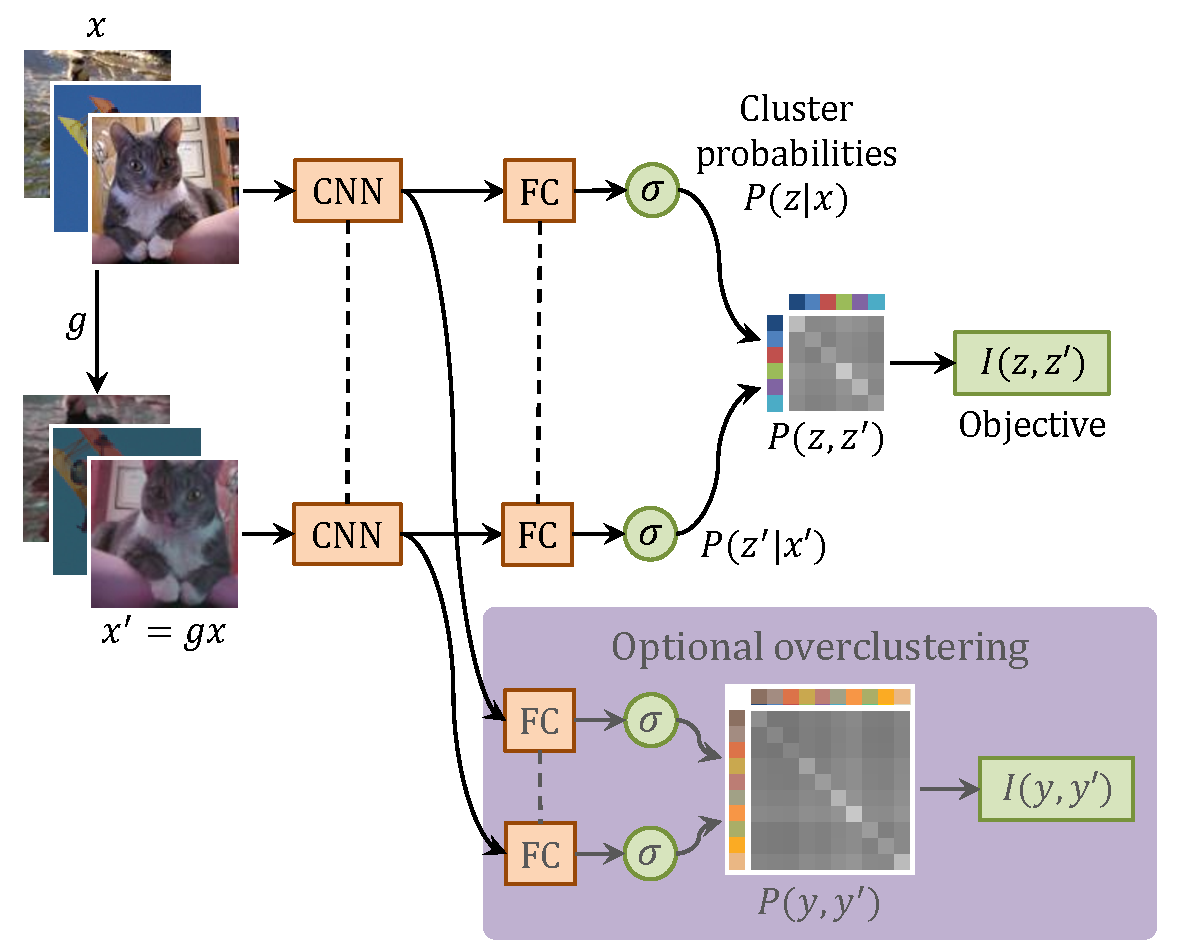
\includegraphics[width=0.95\columnwidth]{paper_imgs/overview1.pdf}
\caption{\label{f:overview}\methodnameshort for image clustering. Dashed line denotes shared parameters, $g$ is a random transformation, and $I$ denotes mutual information~(\cref{e:loss_expanded}).}
\end{figure}


% DAC~\cite{chang2017deep}, JULE~\cite{yang2016joint}, DeepCluster~\cite{caron2018deep}, Associative Deep Clustering~\cite{haeusser18associative} and DEC~\cite{xie2016unsupervised} all rely on the inherent visual consistency and disentangling properties~\cite{greff2015binding} of CNNs to produce meaningful cluster assignments, which are processed and reinforced in each iteration. 
% The latter three are based on using k-means to refine deep feature vectors, a mechanism which is prone to degenerate solutions~\cite{caron2018deep} and thus needs explicit prevention mechanisms such as pre-training, cluster-reassignment or feature cleaning via PCA and whitening ~\cite{xie2016unsupervised, caron2018deep}. 

% DAC is the only unsupervised clustering algorithm out of these that eschews k-means whilst training a network to directly produce cluster assignments, as \methodnameshort does. 
% A network is trained to produce cluster assignment probability distributions for each sample that are used as high level feature descriptors, and the dot product of different descriptors is treated as a proxy for inter-sample semantic distance (instead of Euclidian distance, which is used in the k-means based clusterers). 
% Training proceeds by maximising the dot product of close sample pairs, thus encouraging them to be assigned to the same cluster, whilst minimising the dot product for far pairs. 
% The nature of the optimisation means there is a strong dependency on initialisation and lack of protection against degenerate solutions such as clusters disappearing. 

% \paragraph{Proxy tasks for unsupervised feature learning.}
% For unsupervised feature learning in general, i.e. where the training objective is not clustering, a large number of works explore using proxy learning tasks. 
% There are two major camps:  generative tasks such as autoencoder image reconstruction~\cite{vincent2010stacked}, and spatial-temporal order or context prediction~\cite{lee2017unsupervised,cruz2017deeppermnet,doersch2015unsupervised}. The latter includes predicting patch proximity~\cite{isola2015learning}, solving jigsaw puzzles~(\cite{noroozi2016unsupervised}) and inpainting~(\cite{pathak2016context}). 
% In many cases they benefit from principled formulations that protect against degeneracy.
% However, unlike the aforementioned clustering methods, learned representations from these tasks constitute fine-grained continuous features rather than coarse cluster assignments, and thus must be post-processed, either by unsupervised clustering such as k-means or with label information via SVMs or fine-tuning, in order to produce semantic clusters.

% \paragraph{Invariance as a training objective.}
% Training for function outputs to be persistent through spatio-temporal distortion, noise distortion, or random transforms is an idea shared by \methodnameshort and several mentioned works, including Exemplar CNNs~\cite{dosovitskiy2016discriminative}, IMSAT~\cite{hu2017learning} and proximity prediction~\cite{isola2015learning}.
% It is also seen in Tagger~\cite{greff2016tagger}, which trains a function to denoise its input using several clusters to distribute the representation,~\cite{zou2012deep} which enforces a temporal slowness constraint on learned features, and~\cite{sohn2012learning,hui2013direct} which train for features invariant to local image transformations.




\label{sec:conclusion}
We introduce a novel neural network architecture, the Synchronized Spectral CNN (SyncSpecCNN), for semantic annotation on 3D shape graphs. To share coefficients and conduct multi-scale analysis in different parts of a single shape graph, we introduce a spectral parametrization of dilated convolutional kernels. To allow parameter sharing across related but different shapes that may be represented by very different graphs, we introduce a spectral transformer network to synchronize different spectral domains. The effectiveness of different components in our network is validated through extensive experiments. Jointly these contributions lead to state-of-the-art performance on various semantic annotation tasks including 3D shape part segmentation and 3D keypoint prediction.

\section*{Acknowledgments}
This work is supported by the National Basic Research Program of China (973 program, No. 2014CB340505) and Baidu-Peking University Joint Project.
We thank the Microsoft MSMARCO team for evaluating our results on the anonymous test set. We also thank Ying Chen, Xuan Liu and the anonymous reviewers for their constructive criticism of the manuscript.


% include your own bib file like this:
%\bibliographystyle{acl}
%\bibliography{acl2018}
\bibliography{ref}
\bibliographystyle{acl_natbib}

\end{document}
